\documentclass[lettersize,journal]{IEEEtran}
\usepackage{amsmath,amsfonts}
\usepackage{algorithmic}
\usepackage{algorithm}
\usepackage{array}
\usepackage[caption=false,font=normalsize,labelfont=sf,textfont=sf]{subfig}
\usepackage{textcomp}
\usepackage{stfloats}
\usepackage{url}
\usepackage{verbatim}
\usepackage{graphicx}
\usepackage{cite}
\hyphenation{op-tical net-works semi-conduc-tor IEEE-Xplore}
% updated with editorial comments 8/9/2021

\begin{document}

\title{Evolutionary Multiobjective Surrogate-Assisted Neural Networks for Intrusion Detection in Vehicle Control Area Network}

\author{
         Bin~Cao,~\IEEEmembership{Member,~IEEE,}
         ~Shan~Tian,~\IEEEmembership{}
         ~Malka N. Halgamuge,~\IEEEmembership{Senior Member,~IEEE,}
         ~Saman K. Halgamuge,~\IEEEmembership{Fellow,~IEEE}


\thanks{This work was supported in part by the National Natural Science Foundation of China (NSFC) under Grant No. 61976242, in part by the Natural Science Fund of Hebei Province for Distinguished Young Scholars under Grant No. F2021202010, and in part by the Fundamental Scientific Research Funds for Interdisciplinary Team of Hebei University of Technology under Grant No. JBKYTD2002.

Bin Cao and Shan Tian are with the State Key Laboratory of Reliability and Intelligence of Electrical Equipment, Hebei University of Technology, Tianjin 300130, China; School of Artificial Intelligence, Hebei University of Technology, Tianjin, 300401, China. (email: caobin@scse.hebut.edu.cn; 202022801024@stu.hebut.edu.cn)

Malka N. Halgamuge is with the Cyber Security Research Hub and Department of Computer Science and Information Technology, School of Computing, Engineering and Mathematical Sciences, La Trobe University, Melbourne, Victoria 3086, Australia (e-mail: m.halgamuge@latrobe.edu.au).

Saman K. Halgamuge is with the Department of Mechanical Engineering, School of Electrical, Mechanical and Infrastructure Engineering, The University of Melbourne, Parkville, VIC 3010, Australia (e-mail: saman@unimelb.edu.au). He is also an honorary Professor of the School of Electronics and Information Engineering, Hebei University of Technology, Tianjin 300401, China.

}
}
%\author{Bin Cao, Tian Shan, IEEE Publication Technology,~\IEEEmembership{Staff,~IEEE,}
%        % <-this % stops a space
%\thanks{This paper was produced by the IEEE Publication Technology Group. They are in Piscataway, NJ.}% <-this % stops a space
%\thanks{Manuscript received April 19, 2021; revised August 16, 2021.}}
%
%% The paper headers
%\markboth{Journal of \LaTeX\ Class Files,~Vol.~14, No.~8, August~2021}%
%{Shell \MakeLowercase{\textit{et al.}}: A Sample Article Using IEEEtran.cls for IEEE Journals}

% \IEEEpubid{0000--0000/00\$00.00~\copyright~2021 IEEE}
% Remember, if you use this you must call \IEEEpubidadjcol in the second
% column for its text to clear the IEEEpubid mark.

\maketitle

\begin{abstract}
Modern vehicles are increasingly being equipped with electronic systems making it necessary to ensure their safety and reliability. The most commonly used communication protocol in vehicles, Controller Area Network (CAN) has no direct support for secure communications. In this paper, we propose an intrusion detection model based on a deep neural network with increased accuracy designed using a Multi-Objective Evolutionary Algorithm (MOEA) assisted Neural Architecture Search (NAS). A Graph neural network (GNN) and a convolutional neural network (CNN), both optimized by MOEA are used to explore the internal logical features and spatial features of CAN, respectively. Due to the different functions associated, vehicle CAN messages can have varying lengths. Reinforcement learning (RL) is used to dynamically acquire the lengths of CAN messages and send as samples to the proposed model. A method to convert original CAN data to graph data using its time sequence feature is also proposed. CNN inherits the weights of parents, and GNN inherits the weights of supernet in the evolution process. This weight sharing helps to accelerate the measurement of individual fitness. We apply the proposed intrusion detection model on real-world datasets. While GNN flops are reduced to 40\% of the supernet, the intrusion detection accuracy is increased to more than 95\%. The accuracy of CNN is also improved by 5\% compared to the best individual of the first generation. The accuracy of the intrusion detection achieved by combining the two models is greater than 99\%, which is 4\% better than the model without RL.
\end{abstract}

\begin{IEEEkeywords}
Intrusion Detection of Controller Area Network (CAN), Multi-Objective Evolutionary Algorithm (MOEA), graph neural network (GNN), convolutional neural network (CNN), Neural Architecture Search (NAS)
\end{IEEEkeywords}

\section{Introduction}
\IEEEPARstart{I}{n} the last few decades, the implementation of automotive electronics has experienced rapid growth \cite{1}. This trend has resulted in several changes in the vehicular ecosystem. Drive-by wire (DBW) technology, for example, uses mechatronic systems instead of using mechanical linkages. Control Area Networks (CAN) is considered as a simple and reliable communication protocol and a standard for the in-vehicle networks \cite{2}, connecting multiple electronic control units (ECUs). The adoption of CAN accelerates the applications with the emergence of Vehicle-to-Vehicle (V2V) and Vehicle-to-Infrastructure (V2I) communication interfaces \cite{3}. However, the openness of the vehicular system increases the risk of malicious cyberattacks that can severely threaten human life. Conventional in-vehicle networks are tremendously vulnerable to cyberattacks as CAN was originally developed for an isolated physical system. Every ECU on a CAN bus, for example, can receive any ECU-to-ECU communication. Furthermore, a CAN data packet has no sender’s identification as shown in Fig. \ref{fig_1}. Kwak et al. \cite{KWAK2021114066} conducted several experiments where a CAN message can be readily fuzzed by a packet injection and modification. Various attack scenarios, e.g., disabling brakes and displaying wrong information on an instrument panel (or dashboard), are shown in \cite{5,6}. Attacks on the CAN bus can manifest in several ways. Diagnostic commands deployed during driving can cause malicious effects, e.g., locking the brakes to immobilize the car. However, diagnostic commands should never be displayed when driving normally; thus, they are easily detected. Recent research works \cite{9439954, 9322395} also point to the weakness of security associated with CAN.

\begin{figure*}[!t]
\centering
\includegraphics[width=6in]{figure1_02}
\caption{Typical message injection attack scenarios and the format of CAN. An attacker can inject fabricated messages into the CAN bus of the target vehicle via the on-board diagnostic port of the vehicle or a telematics device that provides a wireless communication channel.}
\label{fig_1}
\end{figure*}

Graph data are widely used in multiple areas \cite{7,8}, for example, used to process Non-Euclidean data features, including in social networks \cite{9}, text networks \cite{10} and biological networks \cite{11}. Graph neural networks (GNN) can be used to solve graph-related problem fields in an end-to-end manner \cite{12}. Relational modeling is crucial for many networks or graphical data mining tasks such as link prediction. GNN has recently been successfully applied in the real world for example in image recognition  \cite{13}, new drug discovery \cite{14} and flow prediction \cite{15}. In their work, the graph data are constructed by the time sequence characteristics of CAN, and the graph neural network extracts the logical characteristics of CAN. However, there are other applications such as social networks or financial networks where more dynamic graphs are used. A dynamic graph can change the nodes of previous graph data or the connection between nodes as time progresses. A graph network can use Recurrent Neural Networks (RNNs) \cite{16, 17} to learn the temporal characteristics of dynamic graphs, and a spatiotemporal graph neural network architecture to learn the spatial characteristics of dynamic graphs \cite{18}. However, some graph data may significantly vary with time and there is very little work to identify the graph network of such graph data. Our approach to construct the graph data of CAN assumes that the nodes or connections of graph data at two time periods may be completely different. Our approach uses a graph collapse network \cite{19} to detect such graph data.

Developing a custom learning architecture consisting of multiple GNN layers for specific scenarios (e.g., biological and physical network data) is difficult even for neural network experts. Falkner et al. \cite{20} pointed out that the deep learning algorithm is very sensitive to many hyperparameters. The work in the literature \cite{21} shows that the hyperparametric optimization (HPO) of GNNs is essential to achieving satisfactory results in practice. Therefore, the study of effective HPO methods is of great value for GNN to be applied to various practical problems. In order to automate the model selection process, neural architecture search (NAS) is widely used in fields \cite{22,23}, and has become the focus of deep learning research in recent years. NAS aims to explore the optimal combination of architecture components from the search space to maximize the model performance applicable to the target problem. So far, there were significant efforts on using NAS to design convolutional neural network (CNN) architectures, which has promoted the latest progress of many important benchmark tasks, such as image classification fields on CIFAR10/100 and ImageNet \cite{24, 25}. In contrast, little work has been done on using NAS for GNN that can learn graphic structure data \cite{26, 27, 28}. NAS literature has proposed two main types of methods as the most effective problem-solving methods: reinforcement learning (RL) and evolutionary algorithm (EA) \cite{29}. So far, EA based NAS methods are not commonly used for designing GNN. The results show that both RL and EA can find equivalent models in terms of accuracy, and EA is faster in some cases \cite{54, 10.1007/978-3-030-61377-8_21}. Two recent related works \cite{28, 30} mainly focus on NAS based on RL and uses RNN as the controller to generate variable-length strings describing GNN architectures that maximize the expected accuracy on the verification dataset. Although encouraging results have been achieved, the existing work has always faced the challenge of the following two shortcomings: hyperparametric invariance and high computational intensity. In addition, the controller usually generates candidate GNN architectures and evaluates them in a sequential manner, which is difficult to expand to large search space.

Generally speaking, a neural network with higher complexity with appropriate regularization in place may have higher recognition accuracy for complex problems. Still, it will significantly increase the detection time of intrusion CAN messages due to higher complexity. NAS can usually be described as a complex optimization problem \cite{29, 31}. Our NAS based method uses two conflicting objectives, namely, the accuracy of intrusion detection and the complexity of the model for multiobjective optimization. In the field of computational intelligence, evolutionary algorithms (EAs) have been widely used to solve various neural network training problems such as weight training \cite{32}, architecture design \cite{33} and learning rule adaptation \cite{34}. EA based methods have been oncreasingly used as NAS optimizers \cite{35, 36, 37}. The GNN gene field \cite{26} uses an EA. It identifies the GNN architecture and trains the hyperparameters in two search spaces, and alternately optimizes the structure and hyperparameters of the graph network (such as learning rate and dropout). Our work combines them into one search space. The recognition rate of the graph network architecture developed by our method is more than 95\%, and the recognition rate of the graph network and convolution network combined is more than 99\%.

Our proposed NAS generates and evaluates the hyperparameter settings iteratively until the preset stop conditions are met to obtain the best solution. Usually, the objective function of a neural network is selected as the fitness function to evaluate the hyperparameters. However, evaluation is typically costly  because training GNN models requires a lot of computing resources. On the other hand, with the development of deep learning, the neural network has a higher number of layers and various other optional hyperparameters (such as activation function and optimization method), which leads to a large search space and increases the difficulty of the search. With the increase of network components, the consumption of computing resources for searching the network is high, and significant efforts are being made for GNN architecture adjustment and optimization. Therefore, a NAS should find the best solution with fewer experiments, reducing the evaluation cost, and improving the exploration ability. Although EAs have competitive search performances in various optimization tasks \cite{38}, as a group-based optimization method, its calculation cost is usually high. This is especially true for EvoNAS, because EAs typically require a large number of fitness assessments, and each fitness assessment in NAS is computationally expensive because it usually involves training deep neural networks from scratch using a large amount of data. For example, an autoencoder based convolutional neural network (AE-CNN) requires 27 GPUs to obtain an optimized CNN architecture on the cifar10 dataset. Some works search the hyperparameters of graph networks and save computing resources by quickly evaluating individuals. For example, \cite{39} proposes parallel graph architecture search to improve search efficiency. In our work, when CNN evolve, offspring inherit the weights of parent networks and GNN inherits the weight parameters of hypernetworks to achieve rapid individual adaptability evaluation.

Deep reinforcement learning is the combination of reinforcement learning and deep learning. This research field can solve a series of complex decision-making tasks that could not be completed by machines before. Therefore, deep RL has opened up many new medical care applications, robotics, smart grid, finance and other fields \cite{40}. The length and content of the CAN messages depend the various functions performed in the vehicle. Based on this inspiration, we use reinforcement learning to obtain the length of the CAN message for each intrusion detection. The experimental results show that the intrusion detection rate of the model increases by 5\% after using the variable-length CAN compared with random length. The reinforcement learning network learns the feature vector of the graph convolution output in each graph network as each state input to the reinforcement learning actor network, and the reinforcement learning outputs the next action, that is, the length of the next CAN message. In early reinforcement learning, there was an overestimation of the real action value \cite{41}, and \cite{42} established two value networks to solve the overestimation problem. Reinforcement learning can be divided into discrete and continuous types according to the types of output actions. The meaning of action in the model is the length of the output CAN messages. We give the range of message length. The integer value between the minimum and maximum length can be taken. Based on the above requirements, we use the TD3 \cite{43} network as a neural network to dynamically obtain the length of CAN messages which are sent to the intrusion detection model every time.

To address the aforementioned challenges, in this paper, we propose a deep neural network intrusion detection model based on evolutionary multiobjective surrogate-assisted neural architecture search to detect CAN intrusion, such as denial-of-service (DoS) and spoofing attacks, with significantly high accuracy and low complicity. In summary, the main contributions of this paper are as follows:
\begin{itemize}
\item{A multiobjective evolutionary GNN detection model is proposed, which takes the detection accuracy and the model flops as the optimization objectives. In the evolution process, the node inheritance strategy is adopted to shorten the time of individual evaluation.}
\item{A method of converting CAN messages into graph data is proposed. Two connected nodes of graph data are constructed according to the timing information of two adjacent timestamps. The logic features in CAN are extracted, so that CAN messages can be classified by GNN.}
\item{A model combining GNN and CNN is proposed to detect CAN intrusion messages, and a reinforcement learning network is used to collect intrusion detection samples of CAN dynamically. During the training of the detection model, the logic and spatial characteristics of CAN are learned simultaneously.}
\end{itemize}

The rest of this paper is organized as follows. Section \ref{section_related_work} introduces the related work of our proposed model. Section \label{section_architecture_search_space} describes the encoding of neural network architectures, followed by the details of the proposed intrusion detection model and the conversion method to graph data from CAN in Section \ref{section_proposed}. Experimental settings and results are presented in Section \ref{section_result}, respectively. Finally, Section \ref{section_conclusion} concludes the paper and proposes some points that can be improved of our model in the future.
\section{RELATED WORK}\label{section_related_work}

\subsection{Conventional intrusion detection of CAN}
A message authentication code, also known as a MAC, is a cryptographic checksum on data that employs a session key to identify unintentional and intentional data modifications. However, the CAN frame is often incapable of supporting MAC \cite{44} and other communication security techniques. Some researchers \cite{45, 46} have attempted to either create new protocols or spread MAC across multiple transmissions. Tashiro et al. establish a method for detecting tampering with individual frames and entire sections \cite{45}. They developed a system that sends a partial MAC in each frame to mitigate against replay, masquerade, and injection attacks. Nowdehi et al. \cite{46} investigate several of these modified protocols based on five industry-specific criteria for prospective CAN message authentication solutions. They discovered that no solution matched all the criteria. VatiCAN employs maintenance support, "adequate implementation details," and no unnecessary overhead, whereas WooAuth modifies the expanded CAN protocol to allow for more authentication codes. Finally, the authors \cite{46} hypothesize that the CAN bus may be "fundamentally unsuitable for secure communication".

\subsection{Deep learning intrusion detection of CAN}
Intrusion detection strategy (IDS) can combine machine learning to train itself to identify abnormal behavior, which can be used as an alternative or supplement to MAC. Spoofing, injection, bus shutdown, and denial of service attacks may all be prevented by intrusion detection systems. Choi et al. introduced voltage IDS in \cite{47}, which uses ECU signal inconsistencies: first performs training and testing, detects the signal characteristics, and then uses the training data to check if the ECU has been compromised. Using multi-class classifiers, one of which corresponds to an ECU, Voltage IDS may identify camouflage attacks. It estimates the most likely sender and compares it to the message's actual CAN ID. A camouflaged attack is identified if they differ. Song et al. \cite{48} solve this problem by changing the ID portion of the CAN frame to binary. For intrusion detection, the updated ResNet model was used to extract the features of the binary text and learn the characteristics of the intrusion message and the regular message. Their experimental findings suggest that their approach outperforms the classic machine learning technique in terms of false-positive rate. Taylor et al. proposed employing deep learning algorithms for intrusion detection in \cite{49} since they are created directly from the network's bit stream. These functions are simple to implement and have a high execution efficiency. While training the characteristics offline, this approach examines the exchange packets in the vehicle network. It responds to the attack in their experiment with a considerably high detection rate.

\subsection{Neural architecture search by EA}
Neural architecture search (NAS) aims to automatically design network architecture, which is essentially an optimization problem of finding an architecture with the best performance in a specific search space with constrained resources \cite{50, 51}. Sun et al. \cite{52} used EA with variable coding length to automatically evolve the architecture of CNN. William et al. \cite{8790093} introduced an evolutionary NAS coding strategy based on directed acyclic graphs (DAG), with better performance than the randomly generated CNN architecture. Real et al. introduced Amoebanet \cite{54}, which employs improved tournament selection to evolve network groups and outperforms the homemade model on Imagenet. Wang et al. \cite{55} designed an effective evolutionary algorithm to optimize the generator within the framework of GANs. This method can effectively improve the generation performance and training stability of the GAN model. Yin \cite{56} uses an evolutionary multiobjective method to design CNN architecture, which uses probabilistic SMBO to maximize classification performance and minimize network reasoning time. Elsken et al. \cite{57} described NAS as a bi-objective optimization problem, in which two objectives are to maximize performance and minimize computing resources. Lu et al. \cite{58} proposed Nsga-net, which can automatically design the network, maximize the model performance, and minimize floating point operations (flops).

\subsection{Surrogate}
A major disadvantage of EvoNAS is that in the process of evolutionary optimization, each new candidate neural network needs to be trained on the training dataset and then evaluated on the validation dataset to avoid over-fitting. Therefore, if the network is large and the training dataset is large, the architecture evaluation in EvoNAS may take several hours. Because EAS is a kind of group-based search method, they usually need a lot of fitness evaluation, making EvoNAS computationally challenging to implement. For example, on CI-FAR10 and CIFAR100 datasets, CNN-GA \cite{59} consumes 35 GPU days and 40 GPU days, respectively, the genetic CNN method \cite{60} consumes 17 GPU days, and the large-scale evolutionary algorithm \cite{61} consumes 2750 GPU days. Therefore, in the case of limited computing resources, the agent model can accelerate the fitness evaluation in EvoNAS. Agents are divided into high-level agents and low-level agents. The high-level agent and low-level agent represent the architecture level and the parameter level in the architecture, respectively. High-level agent representation predicts the accuracy of different neural networks by parameterizing the neural network architecture. However, the low-level agent solves the complexity of using SGD optimization from scratch for each architecture after searching multiple architectures. The low-level agent is given a trained hypernetwork and neural network structure, including all sub architectures. The weight of the neural network architecture inherits the weight from the hypernetwork. In the search process, the accuracy of using the weight inherited from the hypernetwork becomes the standard for selecting the architecture. However, the correlation between the accuracy of prediction architecture and the final accuracy of neural architecture through weight sharing is not close. The neural architecture reference MSuNAS \cite{62} we searched is not only sharing the weight of hypernetwork, but also fine-tuning through training again. MetaQNN \cite{63} uses the agent model to predict the final accuracy of candidate architectures (as time series prediction) from the first 25\% learning curve of SGD training. PNAs \cite{64} use an alternative model to predict the accuracy of the network architecture, adding a branch to the unit structure, which is repeatedly stacked together. Both methods use the agent method to evaluate the performance of neural architecture. However, the correlation between the prediction accuracy of this method and the actual accuracy of the model is relatively low. OnceForAll \cite{65} also uses an agent model to predict the accuracy of architecture coding. However, the agent model is trained offline for the whole search space, so it needs many samples to learn. ChamNet \cite{66} trains many architectures through complete low-level optimization and selects only 300 high-precision samples with different efficiency (trigger, delay, energy) to train alternative models offline. Our model only conducts online learning on samples close to Pareto frontier, which significantly improves the efficiency of architecture search. Our model evaluation method draws lessons from the idea of MSuNAS.

\section{ARCHITECTURE SEARCH SPACE}\label{section_architecture_search_space}
This section introduces the search space of the model, including the search space of GNN and CNN. The search of GCN includes structure and hyperparameter search. The structure search includes the number of layers of the GCN layer and the width of the prediction layer of the graph network. Hyperparameter search includes learning rate, activation function type, dropout rate, etc. CNN \cite{48} architecture of our model consists of one stem part and four Res CNN block parts. The CNN part of our model retains the stem part and extracts eight positions on the four Res CNN blocks. There are five options for each of these eight locations.

\subsection{GNN architecture search}
The specific genes and corresponding relationships are shown in Table \ref{table1}. The chromosome is divided into nine parts. The first part of the chromosome is position 0. A gene indicates There is a gene indicating whether to use the direction information of graph data constructed by CAN IDs. The graph data can determine the direction of the edge of the directed graph according to the sequential relationship between two adjacent frames. Specifically, the CAN IDs of the previous frame points to the next frame. Although using the direction of constructing graph data will make more use of the information of graph data, the experimental results show that using more graph information does not necessarily improve the recognition accuracy. See the next section for the analysis of specific experimental results. According to the formula in the previous section, it is necessary to obtain the Laplace matrix of each subgraph and calculate the eigenvector of each subgraph. Whether to use regularization for the Laplacian matrix before calculating the eigenvector of each subgraph. The regularized Laplacian matrix $L_{norm}$ and the nonregularized Laplacian matrix L of the graph network are expressed as

\begin{equation}
\label{deqn_ex_7}
L\ =\ D\ -\ A
\end{equation}

\begin{equation}
\label{deqn_ex_8}
L_{norm}\ =\ I\ -\ D^{-1/2}AD^{1/2}
\end{equation}

where A represents the adjacency matrix of graph data and D represents the degree matrix of graph data. The third part of the chromosome, positions 2 to 3, is the depth of the two GCN blocks. One GCN block is laid before graph coarsen, and the one is laid after graph coarsen. The fourth part of chromosome, positions 4 to 5, is the number of neurons in each layer of the prediction layers. In the process of evolutionary algorithm search, the neural network architecture refers to \cite{62, 67}, are dynamically changed. The appropriate number of layers of graph convolution and the number of neurons in the prediction layer can achieve good detection accuracy while the complexity is not high. Parts 5 to 7 of chromosome, positions 6 to 8, represent the hyperparameters in the network architecture, such as dropout rate, learning rate, etc. Chromosome Part 8, positions 9 to 10, respectively represent how to reduce the dimension into a one-dimensional vector after each convolution block outputs the convolution result. There are three options: sum, average and maximum for each dimension. Part 9 of chromosome represents the activation function after the end of convolution or FCNN.

\begin{table*}[!t]
\caption{GNN search space\label{table1}}
\centering
\begin{tabular}{cccc}
\hline
Part & Position & Meaning	 & Search space\\
\hline
1 & 0 & directed/undirected graph & directed undirected\\
2 & 1 & Whether Normalization of subgraph & not normalization normalization\\
3 & 2-3 & Layers of GCN & one two three\\
4 & 4-5 & Proportion of neurons in prediction layer & 0.25 0.5 0.75 1.00\\
5 & 6	 & Dropout & 0.005 0.01 0.02 0.03 00.4 0.05\\
6 & 7 & Weight Decay Rate & 5e-4 8e-4 1e-3 4e-3\\
7 & 8	 & Learning Rate & 5e-4 1e-3 5e-3 1e-2\\
8 & 9-10 & way to merge the vectors of every GCN layer & sum average max\\
9 & 11-18 & Activation function & sigmoid tanh relu  leaky\_relu relu6\\
\hline
\end{tabular}
\end{table*}

\subsection{CNN architecture search}
CNN, such as the variants of Inception and ResNet, are designed to build neural networks by stacking multiple blocks. The neural network architecture design includes the determination of depth (number of layers), width (number of channels) and spatial resolution change (number of pool layers), while the block structure design specifies hierarchical connection and local calculation. Through this block design method, the generated model can not only achieve high performance, but also be extended to different datasets and tasks.

An operation space is defined by a set of possible basic components of network architecture and known successful modules designed by human experts. The five operations used in this work and the corresponding genotype-phenotype mapping are shown in Table II. In the table, spatial separable convolution (SP) and deepwise separable convolution (DW) can reduce network parameters without sacrificing network performance. Here, we use two DW operations and two SP operations, and the kernel size respectively is 3 × 3 and 5 × 5, referred to as SP3, DW3 and SP5, DW5.

\begin{table}[!t]
\caption{CNN search space\label{table2}}
\centering
\begin{tabular}{cccc}
\hline
Operation type & Kernel size & Short name & Code\\
\hline
Spatial Separable Convolutions	 & 3 & SP3 & 0\\
Spatial Separable Convolutions	 & 5 & SP5 & 1\\
Depthwise separable convolution & 3 & DW3 & 2\\
Depthwise separable convolution & 5 & DW5 & 3\\
Normal convolution & 3 & 3*3 & 4\\
\hline
\end{tabular}
\end{table}


\section{PROPOSED INTRUSION DETECTION MODEL}\label{section_proposed}
The architecture we proposed is shown in the FIg. \ref{fig_2} and can be divided into two parts of requiring CAN part and intrusion detection part. Requiring CAN part is constructed by reinforcement learning (RL) network to dynamically collect CAN messages. Intrusion detection part is constructed by GNN and CNN. The network architecture of GNN and CNN is optimized by EA. The parts optimized by EA are marked with dotted lines in the Fig. \ref{fig_2}. They are the convolution layer of CNN, the GCN layer of graph neural network and the full connection layer etc. At the same time, using the advantages of two different neural networks, GNN has the advantage of extracting logical features and CNN has the advantage of extracting spatial features. Finally, the output results of the two networks are integrated to obtain the final result. Both GNN and CNN are binary-class networks, before the final output of the intrusion detection results, it is judged that the output of each network has one row and two columns of vectors, and the output is the network result with a larger difference between the two columns of the two network output vectors.

\begin{figure*}[!t]
\centering
{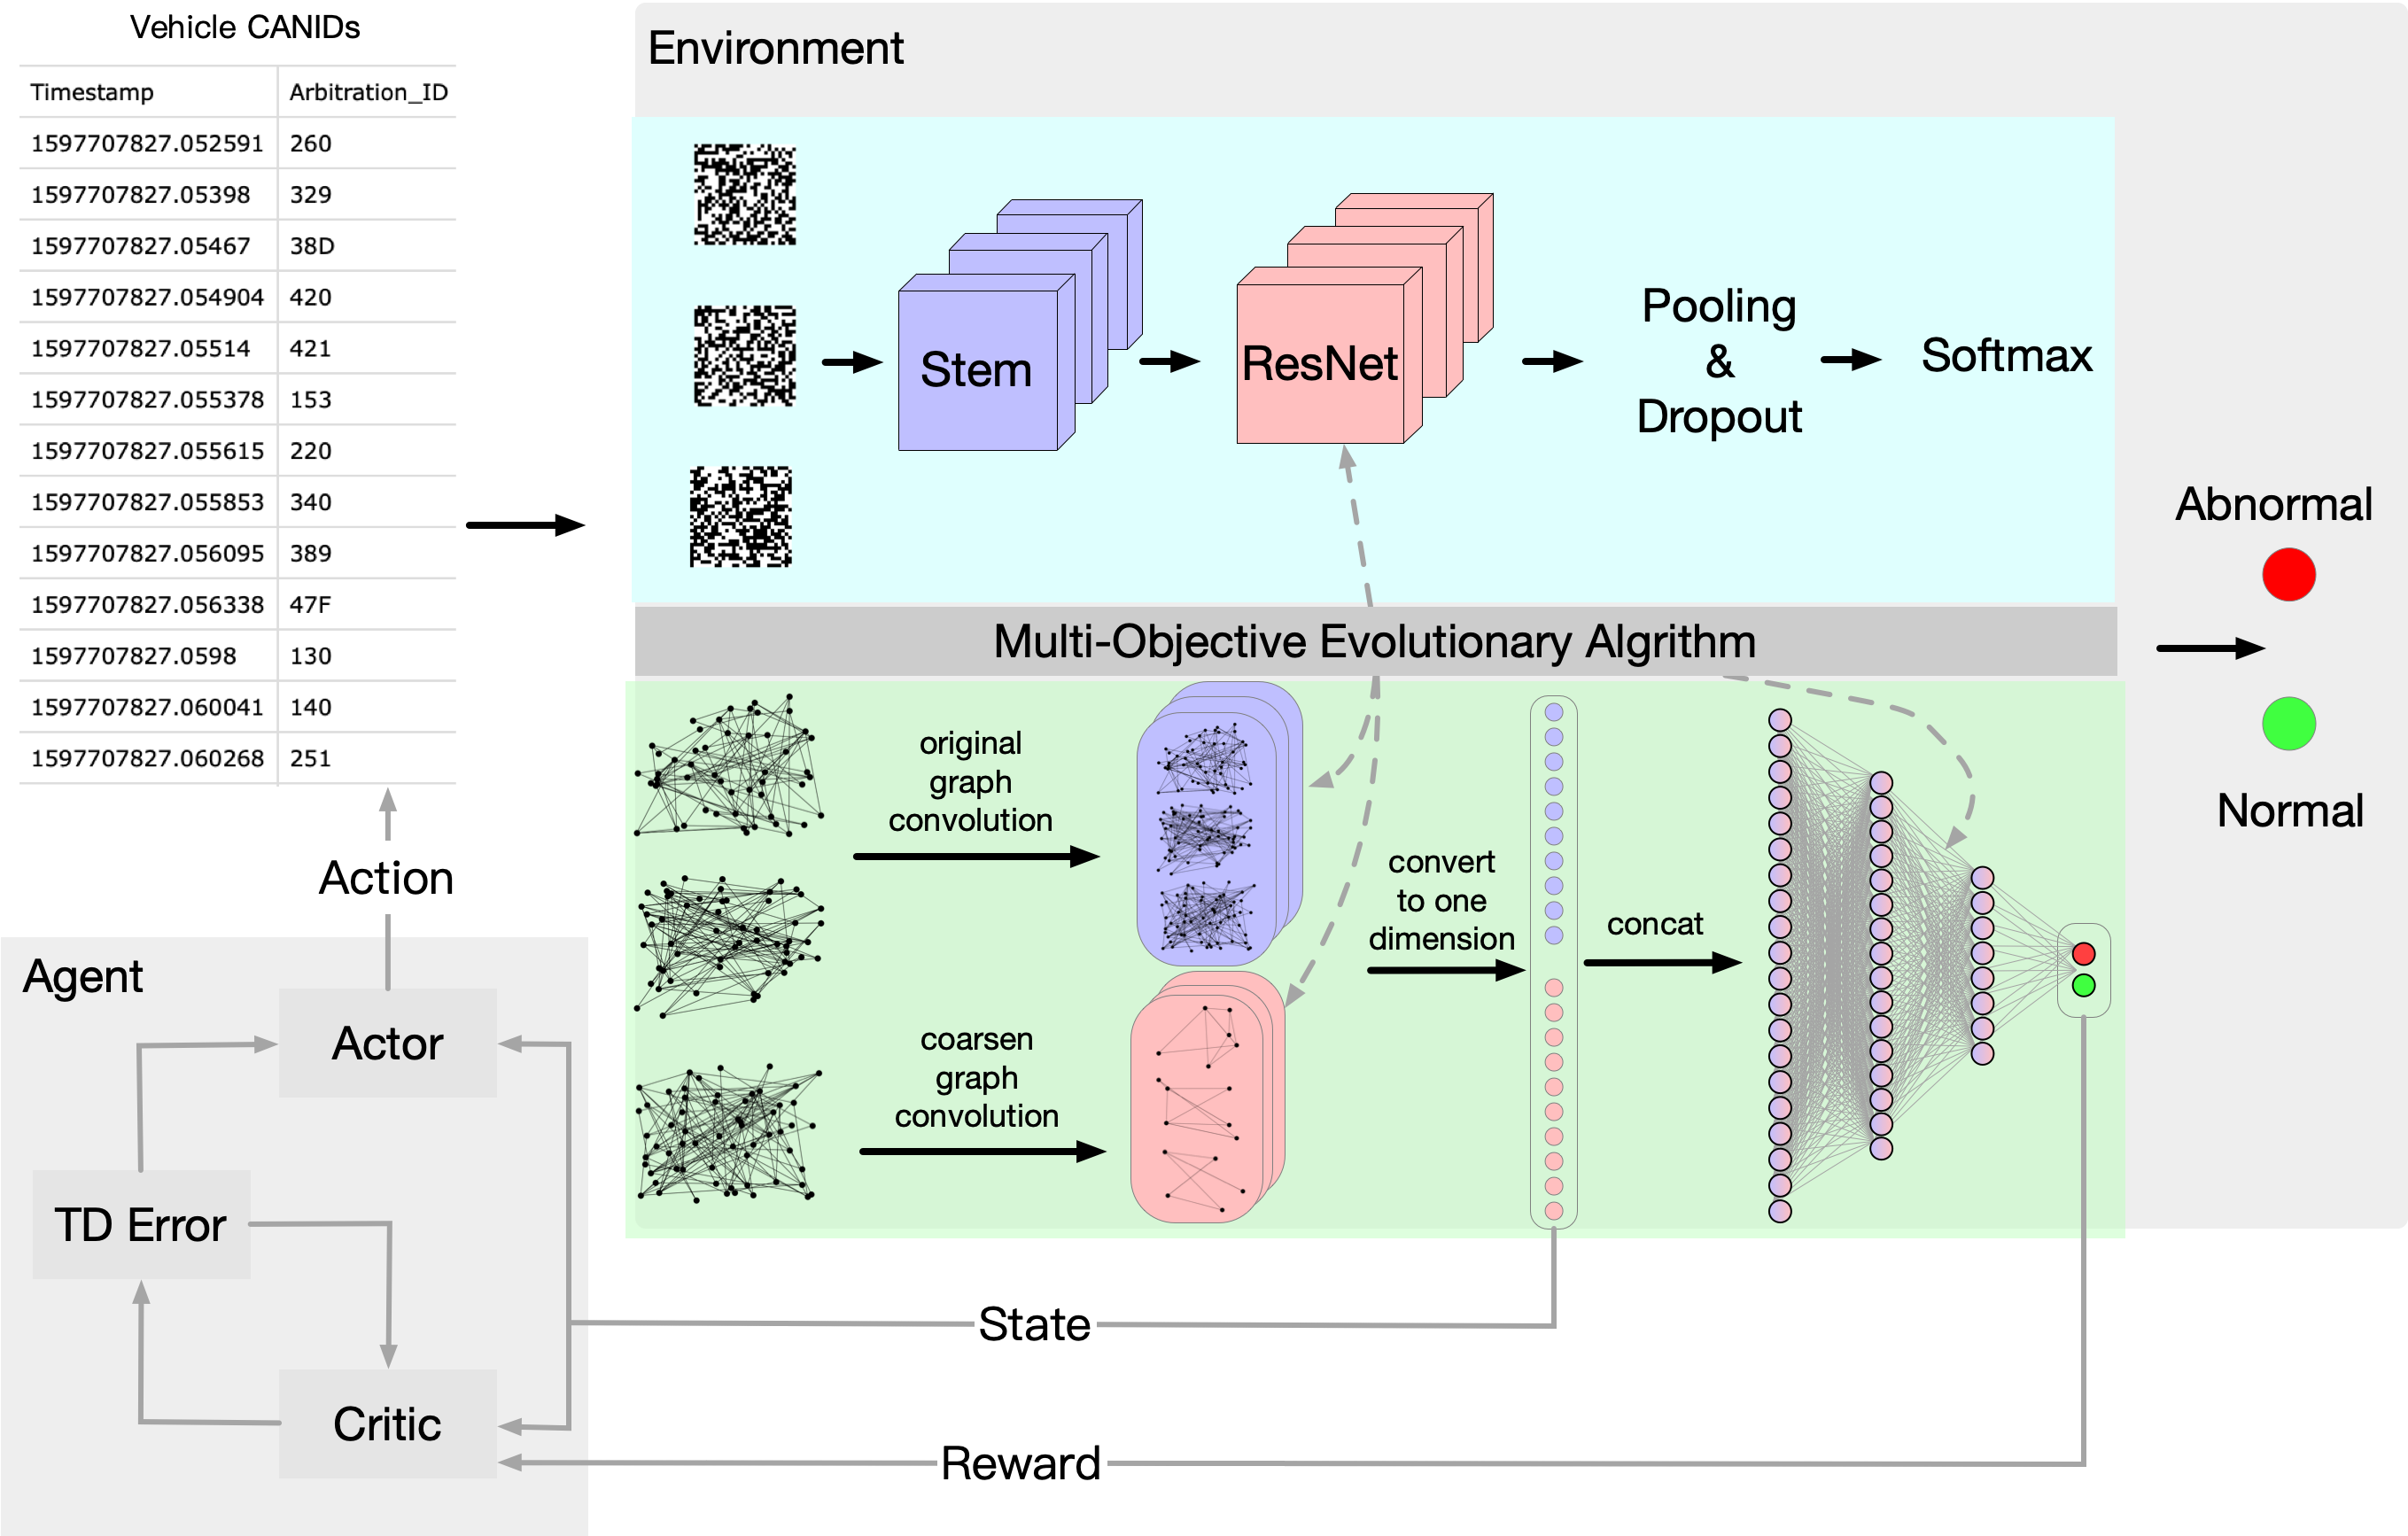
\includegraphics[width=7in]{evo-frame}%
\label{Overall framework of network architecture.}}
\hfil
\caption{Overall framework of network architecture. The samples of CANID sent to intrusion detection model is illustrated in the upper right corner of the figure. The CAN intrusion detection part of our model is the environment of RL and it’s in the largest gray box on the right. The RL’s agent is composed of FCNN, which is in the gray box on the lower left. The detection part consists of CNN and GNN. CNN is on the blue background above and GNN is on the green background below. Both CNN and GNN are optimized using MOEA algorithm. The dotted line in the figure points to the optimized part from the dark gray box of MOEA in the middle. The optimized part in CNN includes the RESNET structure and hyperparameters, such as learning rate, dropout, etc. The optimized part in GNN includes the number of GCN layers, the number of neurons in each layer of the FCNN and hyperparameters, such as learning rate, dropout, etc. The design details of RL, GNN, CNN are described in \ref{RL}, \ref{GNN}, \ref{CNN}.}
\label{fig_2}
\end{figure*}

\subsection{Collect CAN by Reinforcement Learning (RL)}\label{RL}
RL network is able to dynamic collect CAN messages of every detect sample which will send to GNN and CNN. Before each intrusion detection, the length of one of the CAN messages is collected as a sample input to the detection network. In the vehicle CAN message, the message data of different functions or the message of the same function need different frames to complete, so the RL network is used to solve the problem of dynamic acquisition of CAN messages of different lengths. Before training RL network, a GNN with intrusion detection ability is trained first. When training the GNN, the length of input is generated randomly. There are two convolution layers in this GNN. The output of the convolution layer of GNN is converted into one-dimensional vectors, and the two one-dimensional vectors are combined as the state input of RL network. The reward function is designed by using the recognition results at the out of the flattened layers of GNN. If the GNN graph network recognition is correct, it will get a positive reward, and if the recognition is wrong, it will get a negative reward or penalty. The RL network architecture design of this work refers to Twin Delayed Deep Deterministic Policy Gradients TD3 \cite{43}. To avoid overestimation of value network, RL network is composed of two value networks and two action networks, and the output is discrete. The dimension of reinforcement learning network output is the difference between the maximum CAN length and the minimum CAN length of intrusion detection is given by

\begin{equation}
\label{deqn_ex_1}
%x = \sum_{i=0}^{n} 2{i} Q.
\footnotesize {{output\_dim}_{RL}\ =\ MAX(CAN\_LEN)\ -\ MIN(CAN\_LEN)}
\end{equation}

\subsection{Intrusion detection by Graph Neural Network (GNN)}\label{GNN}

Here are our design assumptions for the proposed intrusion detection model. We assume:

\begin{enumerate}
\item{each ECU also runs intrusion detection software that monitors and identifies intrusions in the in-vehicle network.}
\item{intruder can gain physical or remote access to the CAN bus via an exposed interface, such as vehicle to everything (V2X), entertainment systems, or advanced driver assistance systems (ADAS), either physically via the OBD-II port or remotely via Bluetooth, WiFi, or telematics services, such as 3G and long-term evolution (LTE).}
\item{raw payload bit decoding into signal values has already been completed.}
\item{attacker attempts to manipulate communications in order to affect the vehicle's behavior.}
\item{attacker can shut off any ECU and/or insert malicious messages arbitrarily.}
\end{enumerate}

First, we set the previous frame of CAN message to point to the next frame. Because the number CANIDs are limited, not all CANIDs will point to a new CANID, it may also point to a CANID that has appeared before. The direction relationship of the converted graph data is related to the time sequence of the CAN frame sequence. A sequence of CAN IDs always indicates different functions in the vehicle, and whether the logic of the execution sequence of the functions is reasonable or not can be learned by the GNN. For example, it can learn a large acceleration signal appearing when braking, or a vehicle ignition signal appearing without a car key signal is not reasonable. It is then very likely that an intrusion message has appeared on the CAN bus, which has practical significance. For the GNN to learn more abstract features, we input a partial graph of sequence data to determine whether the message is an intrusion message, instead of inputting one or two frames of message. Our proposed approach is shown in Fig. \ref{fig_3}.

\begin{figure*}[!t]
\centering
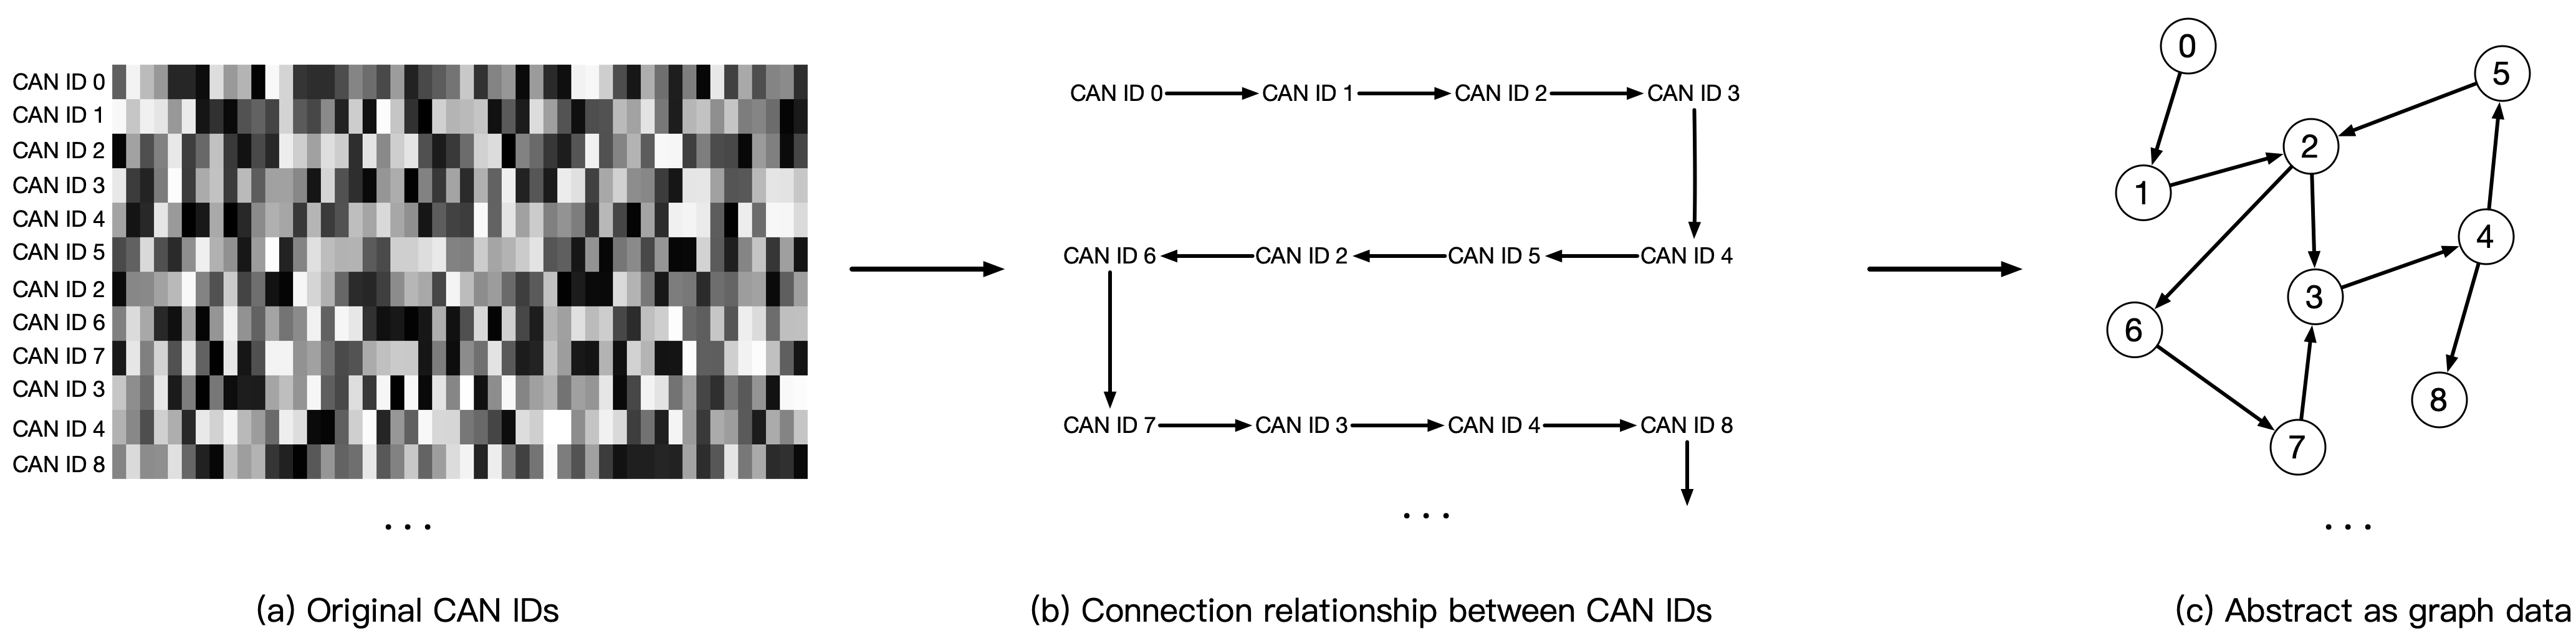
\includegraphics[width=7in]{graph-data}
\caption{Construct graph data from original CAN.}
\label{fig_3}
\end{figure*}

The GCN performs a in this work is a graph level classification task, and the network architecture of GCN is inspired by graph classification task refers to \cite{19}. The main idea of the GNN of our model is to perform graph convolution on the original graph and the pooled graph respectively through graph convolution network (GCN), convert the results of the two GCN into two one-dimensional vectors, combine the two one-dimensional vectors and send them to the fully connected neural network (FCNN) to complete the detection task. The work in \cite{19} is dividing the  node of graph into several clusters. Each cluster can be regarded as a subgraph of graph data to obtain the eigen matrix of a series of subgraphs. Using eigenvectors to construct the pooling matrix, each subgraph is pooled into a super node.  Graph $G$ connected by given $K$ subgraphs, $C$ is a part of $G$. $N_k$ represents the number of nodes in the subgraph $G^{(k)}$. $\Gamma^{\left(k\right)}$ is the list of nodes in the subgraph $G^{(k)}$. Each subgraph can be regarded as a super node of graph $G$. Define sampling operator $C^{\left(k\right)}\in\mathbb{R}^{N\times N_k}$ as follow:

\begin{equation}
\label{deqn_ex_2}
C^{\left(k\right)}\left[i,j\right]=1\ if\ and\ only\ if\ \Gamma^{\left(k\right)}\left(j\right)=\upsilon_i
\end{equation}

where $C^{\left(k\right)}\left[i,j\right]$ represents the element in $i-th$ row and $j-th$ column of $C^{\left(k\right)}$, $\Gamma^{\left(k\right)}\left(j\right)$ represents the $jth$ node in the node list $\Gamma^{\left(k\right)}$. This operation indicates the correspondence between the node in the subgraph $G^{(k)}$ and the original graph $G$. Because Fourier transform can convert the graph signal to the frequency domain and take the signal information and the structure information of graph data into account, we refer to as in [19], we use Fourier transform to design pooling operation. The pooling operation pools the constructed graph signal $G$ into $G_{coar}$. Pooling operation is based on the Fourier transform of each subgraph ${{G^k}}_{k=1}^K$. The Laplace matrix of the subgraph $G^{(k)}$ is $L^{(k)}$. $u_1^{(k)}, …, {\ u}_{N_k}^{(k)}$ represents the all eigenvectors of the Laplacian matrix $L^{(k)}$ of the $k-th$ subgraph. Then use the upsampling operation $C^{(k)}$ to upsample the eigenvector to the whole graph $G$. The upsampling equation is represented by

\begin{equation}
\label{deqn_ex_3}
{\bar{u}}_l^{(k)}=\mathbf{C}^{(k)}\mathbf{u}_l^{(k)},l=1\ldots N_k
\end{equation}

$\Theta_l\ \in\ \mathbb{R}^{N\times K}$ represents the pooling matrix containing the L-th eigenvector of all subgraphs.
where $\Theta_l\ \in\ \mathbb{R}^{N\times K}$ represents the pooling matrix containing the $L-th$ eigenvector of all subgraphs is given by

\begin{equation}
\label{deqn_ex_4}
\mathrm{\Theta}_l=\left[{\bar{u}}_l^{\left(1\right)},\ldots,{\bar{u}}_l^{\left(k\right)}\right].
\end{equation}

Each subgraph does not necessarily have the same number of nodes, that is, the number of eigenvectors of each subgraph is not necessarily equal. $N_{max}\ =\ \underset{k\ =\ 1,...,K}\max{N_k}$ represents the maximum number of nodes in all subgraphs. For the subgraph $G^{(k)}$ owns $N_k$ nodes, the lst pooling operation is expressed as:

\begin{equation}
\label{deqn_ex_5}
X_l\ =\ \mathrm{\Theta}_l^TX
\end{equation}

where $X_l$ indicates the result of the L-th pooling operation. The k-th row of $X_l$ contains the information of the k-th subgraph, that is, the k-th super node. Based on the above structure, we can construct $N_{max}$ times of pooling operation, and combine the results of all pooling operations to form the coarsen matrix shown as:

\begin{equation}
\label{deqn_ex_6}
X_{coar}\ =\ [X_0,...,X_l,\ ..X_{N_{max}}].
\end{equation}

In some other graph classification tasks using pooling method, the sum or average method is used to treat each node in the subgraph indiscriminately, and the structure information of nodes in each subgraph cannot be extracted. In our work, we pool the graph data once, and apply a GCN operation to extract features before and after pooling. Finally, the outputs of the two graph convolutions are transformed into one-dimensional vectors by summation or averaging, and the two one-dimensional vectors are merged into a single to the FCNN layers for classification.

The crossover and mutation operations of the GNN are shown in Fig. \ref{fig_4} and \ref{fig_5}. The crossover operation is to select two parents randomly in the population, and then randomly select the crossover point on each parent, and the separated parts are exchanged to generate two new offspring individuals. Mutation operation is to select a parent in the population with mutation probability, and then randomly select the mutation point on the parent to cause gene mutation.

\begin{figure*}[!t]
\centering
\includegraphics[width=7in]{gnn-cross}
\caption{GNN crossover operation.}
\label{fig_4}
\end{figure*}

\begin{figure*}[!t]
\centering
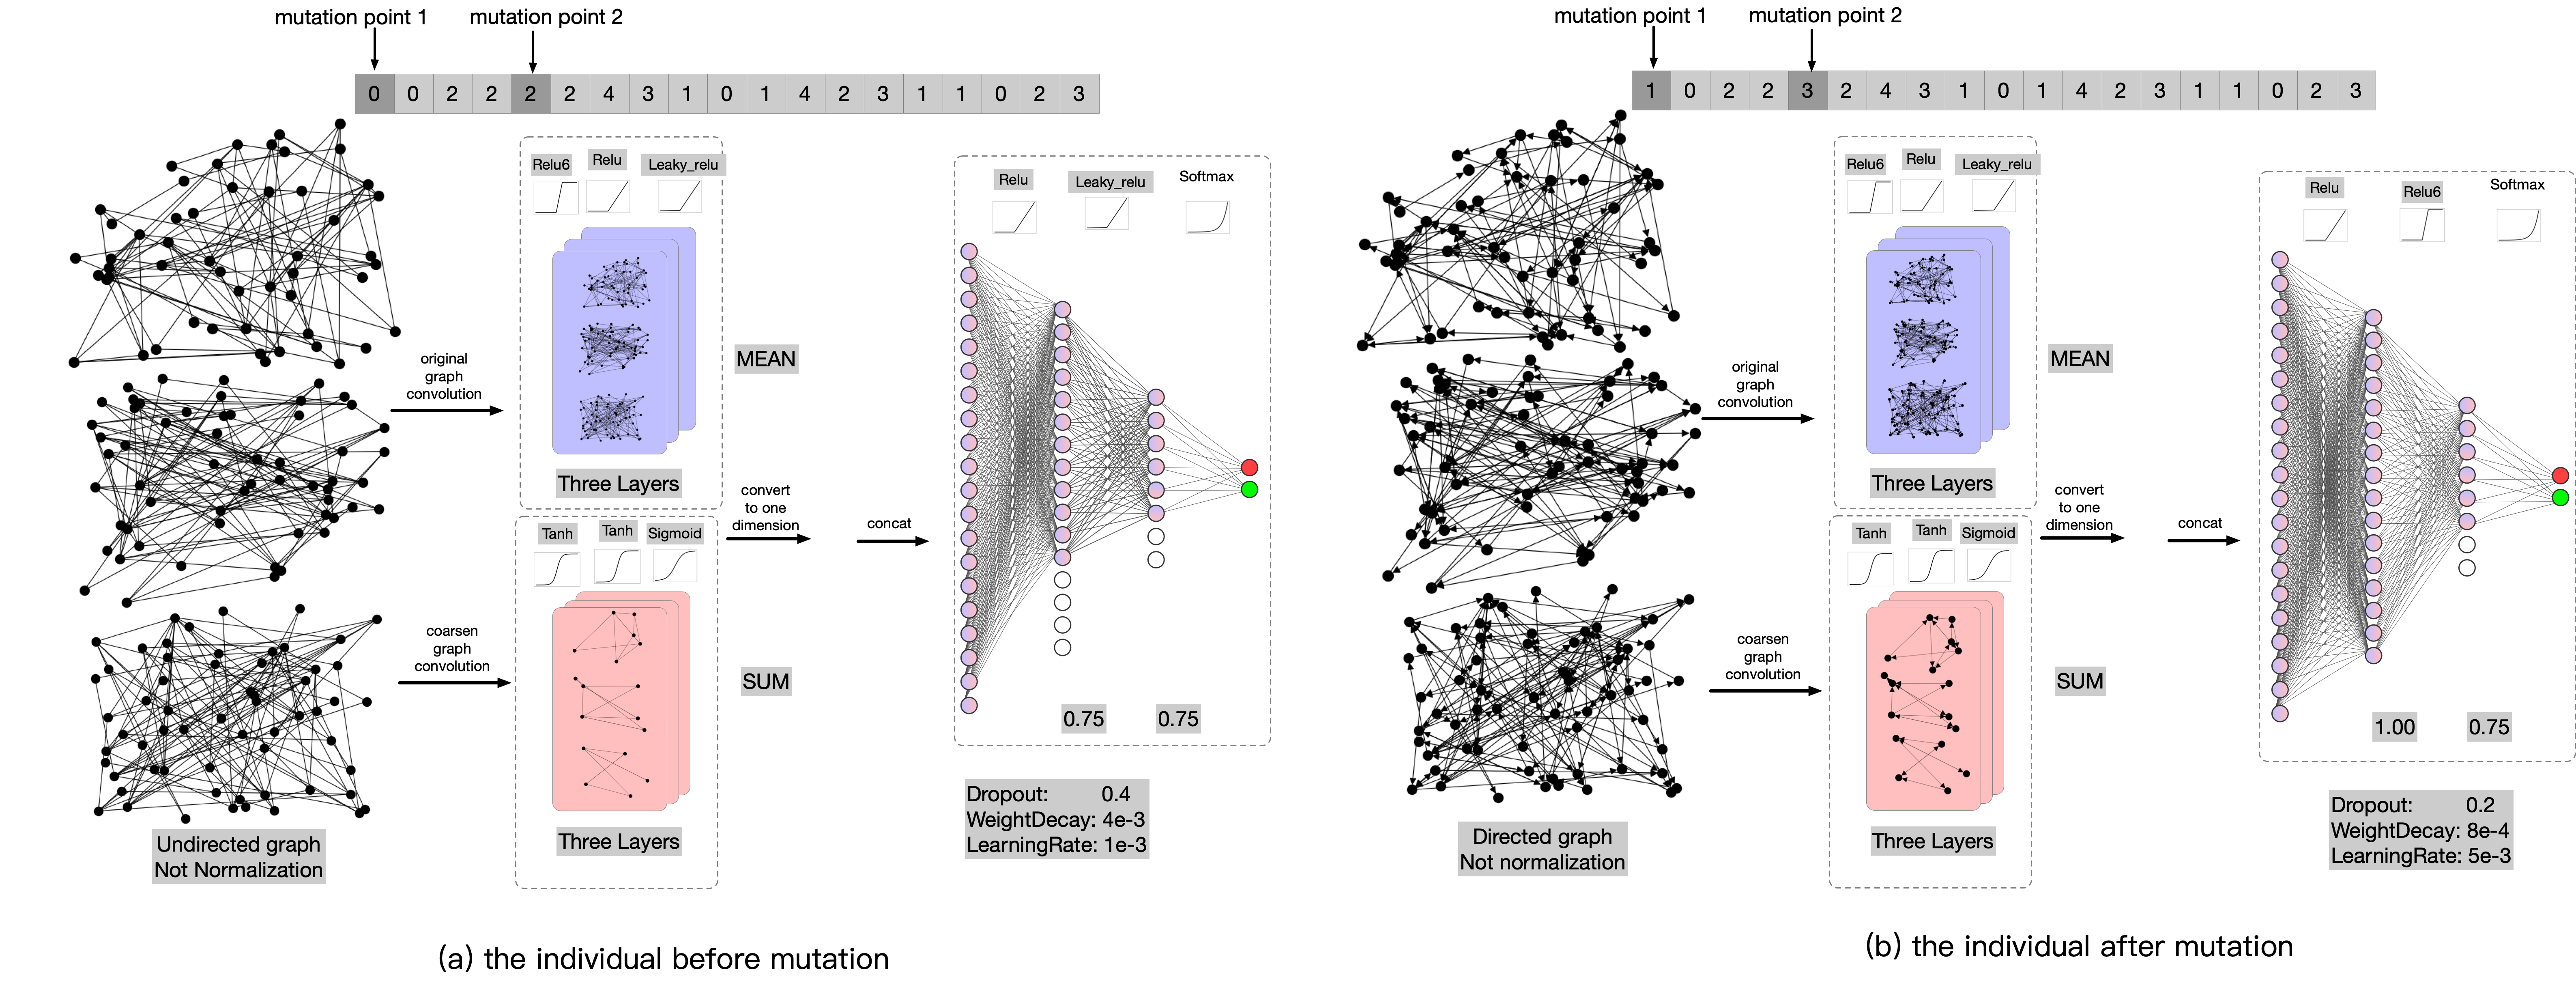
\includegraphics[width=7in]{gnn-mutation}
\caption{GNN mutation operation.}
\label{fig_5}
\end{figure*}

\subsection{Intrusion detection by convolutional neural network (CNN)}\label{CNN}

The hexadecimal CAN IDs are transformed into binary to form a sample similar to an image. Each pixel is 0 or 1 respectively. According to the reference paper \cite{48}, the number of ID bits of vehicle CAN extended frame is 29 bits, and 29 frames are collected to construct 29 × 29 samples. Through the processing of samples, the detection task is transformed into a task similar to image classification.  We follow the same block level design method as in \cite{68, 69, 70}. Block is a small convolution network. To deal with different intermediate information more effectively in forward propagation, four kinds of convolution blocks, shown in Figure 6, are designed according to the different grid sizes of feature mapping. At the same time, the reduction block is designed to increase the deep receptive field, and halve the grid size of the feature map by applying all operations in steps of 2. According to the Convention of modern CNN Architecture \cite{71, 72, 73}, when the grid size of the feature graph is halved, we double the number of channels (filters) of the block to maintain a roughly constant hidden state dimension.

Inception ResNet is a kind of deep convolution model. It is designed to divide images into 1000 categories in the field of image classification and shows promising performance. The overall architecture of the CNN is shown in Figure 6. The input size is $29\times29\times1$, and the input data size is converted to $13\times13\times28$ through the stem module. After the four modules optimized by EA, the data size is $2\times2\times896$. Finally, the data is transformed into a binary classification vector with of two dimensions through the softmax module. The whole convolution network architecture is shown in Fig. \ref{fig_6}. 

\begin{figure*}[!t]
\centering
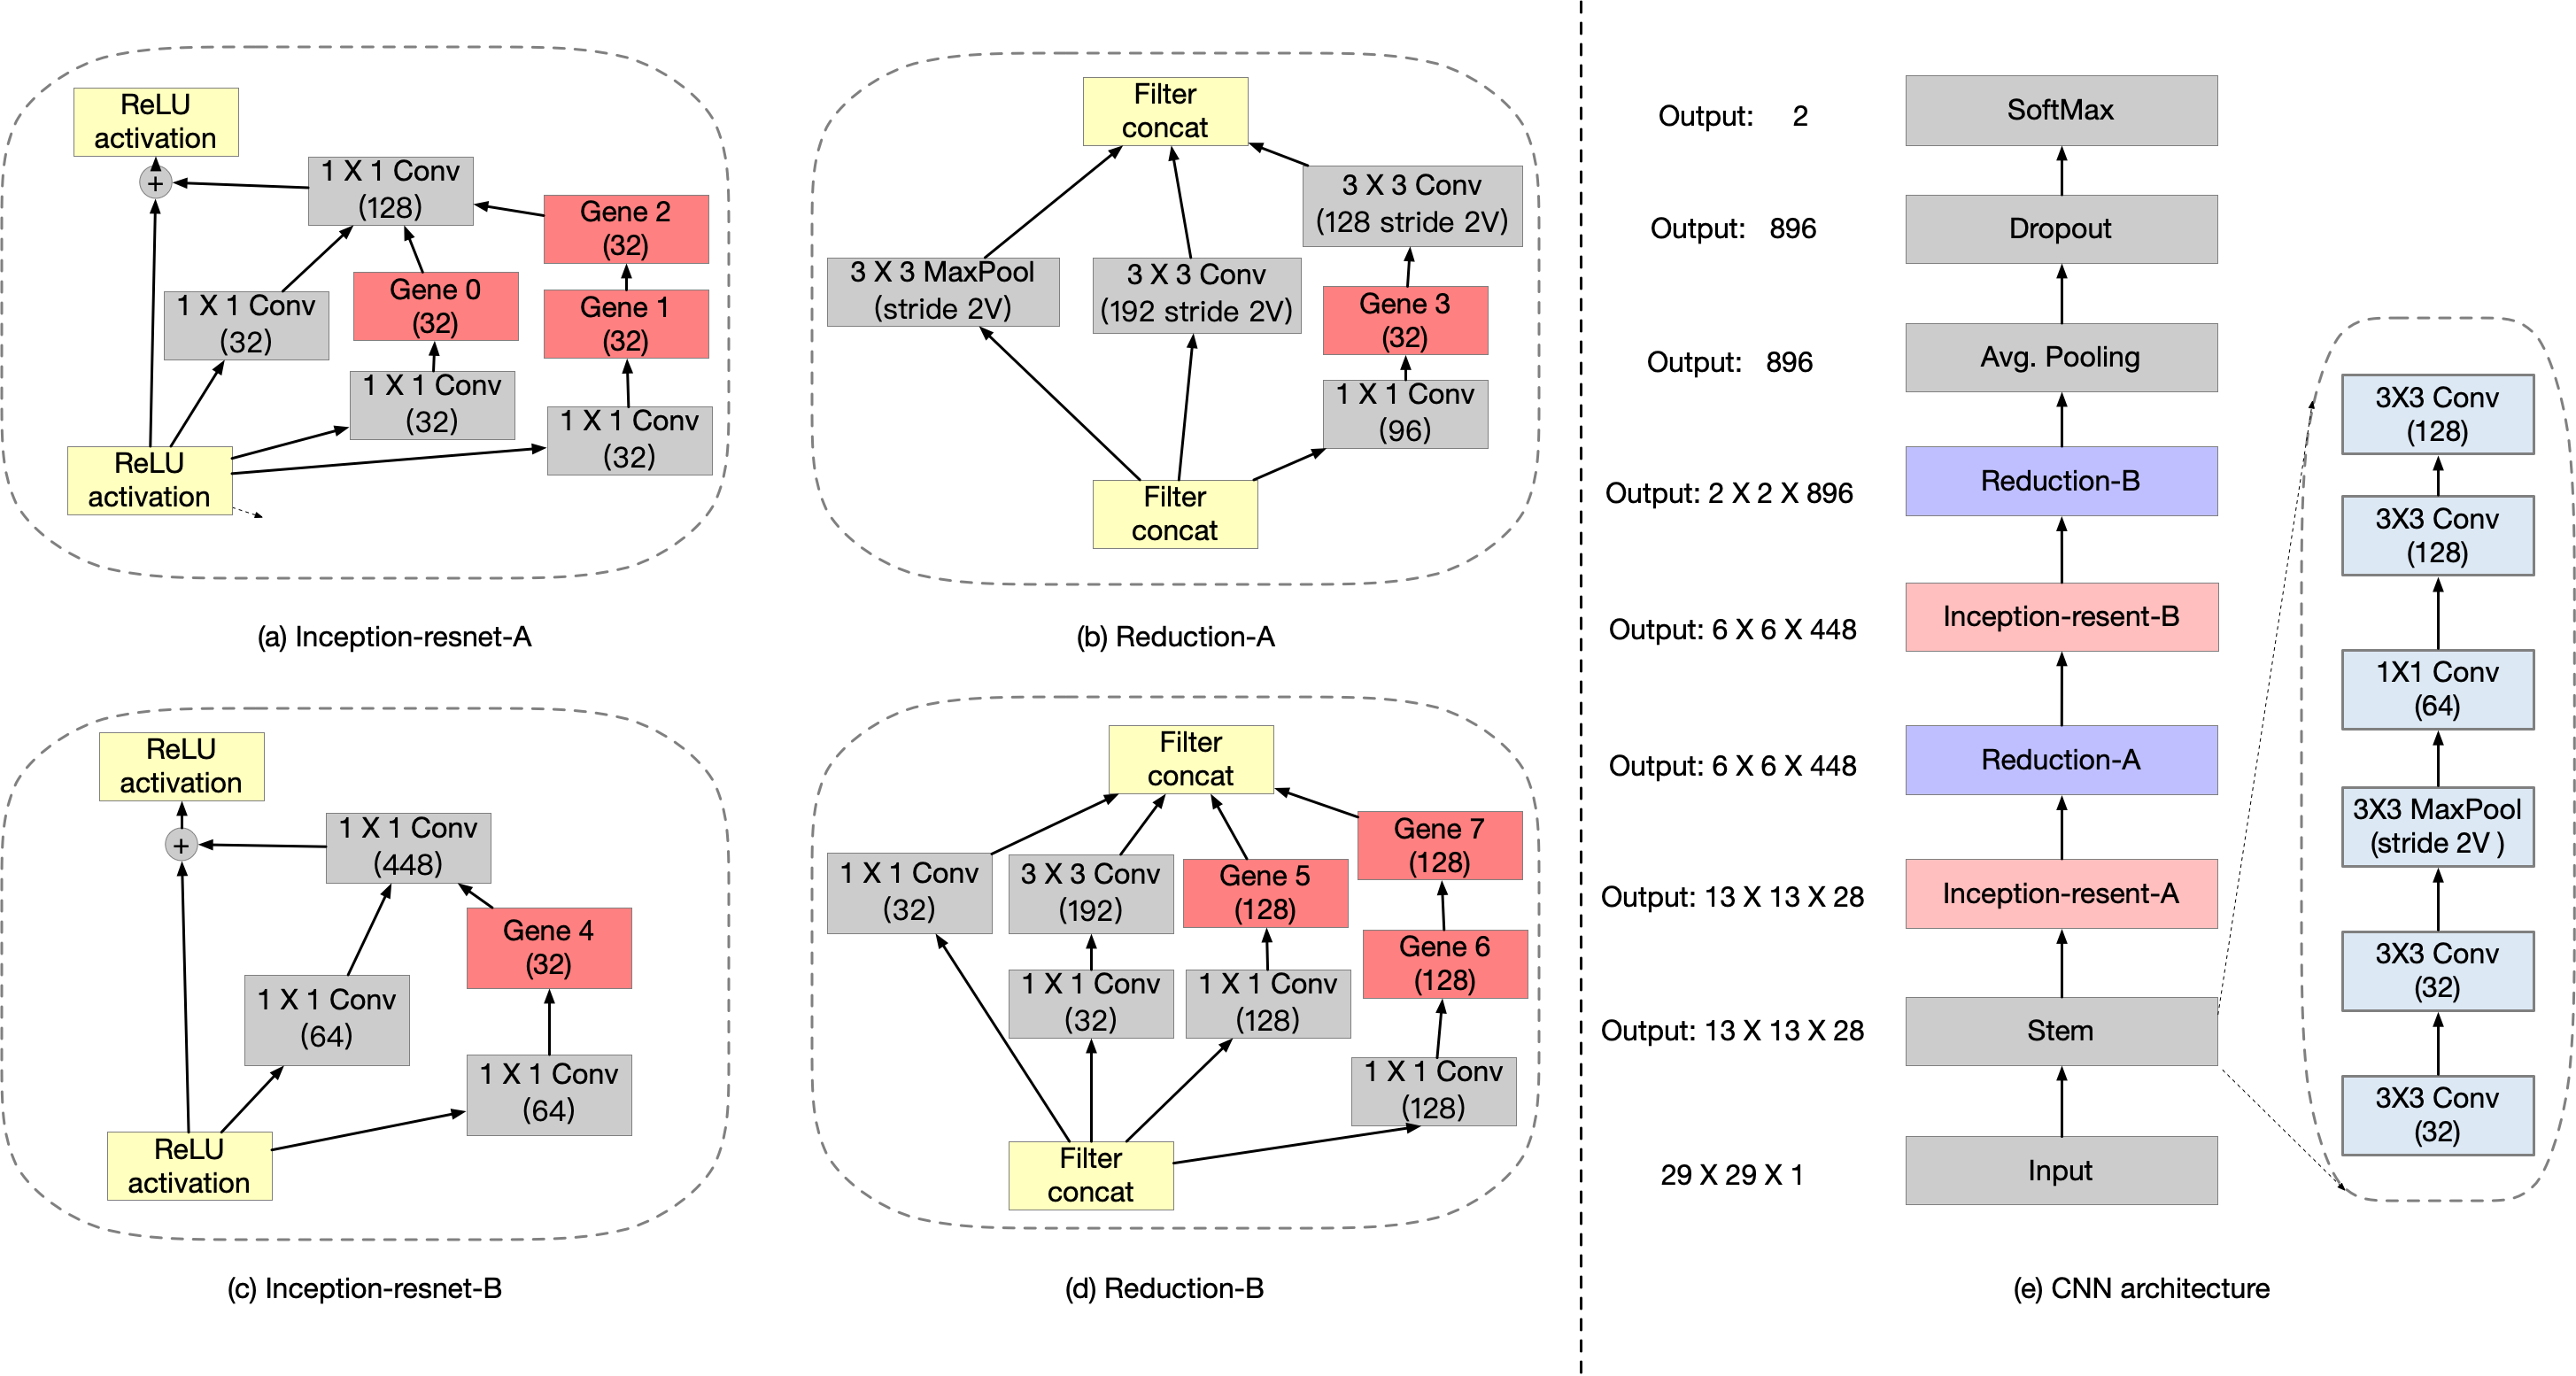
\includegraphics[width=7in]{cnn-overall}
\caption{Res-Inception blocks of CNN.}
\label{fig_6}
\end{figure*}

Because an individual is retrained every time, the amount of calculation required is normally extensive even for a small population of individuals. To improve the evaluation efficiency of MOEA, an agent is used to exchange the weight parameters of corresponding neural network positions in the process of crossover operation and mutation operation. It can be seen from the schematic diagram that channels in each convolution block are different, and the number of gene channels in each convolution block is the same, which has no impact on the crossover operation, but will affect the mutation operation. At two gene exchange positions on the parent chromosomes, the corresponding weights of the neural network need to be exchanged, so the number of channels of the two genes needs to be the same. Both RedA and ResB convolution blocks have only one gene, and ResA and RedB convolution blocks have three genes respectively. Therefore, mutation can only be performed in ResA block or RedB block. The crossover operation of evolution part first takes out two parent individuals by the tournament selection method with n=2, then randomly selects the intersection on each parent, disconnects at the intersection, and exchanges the separated parts to generate two new offspring individuals. The crossover process is shown in Fig. \ref{fig_7}. Mutation operation is to mutate each parent with mutation probability $p$, and then randomly select two points on the parent to exchange. The mutation process is shown in FIg. \ref{fig_8}.

\begin{figure*}[!t]
\centering
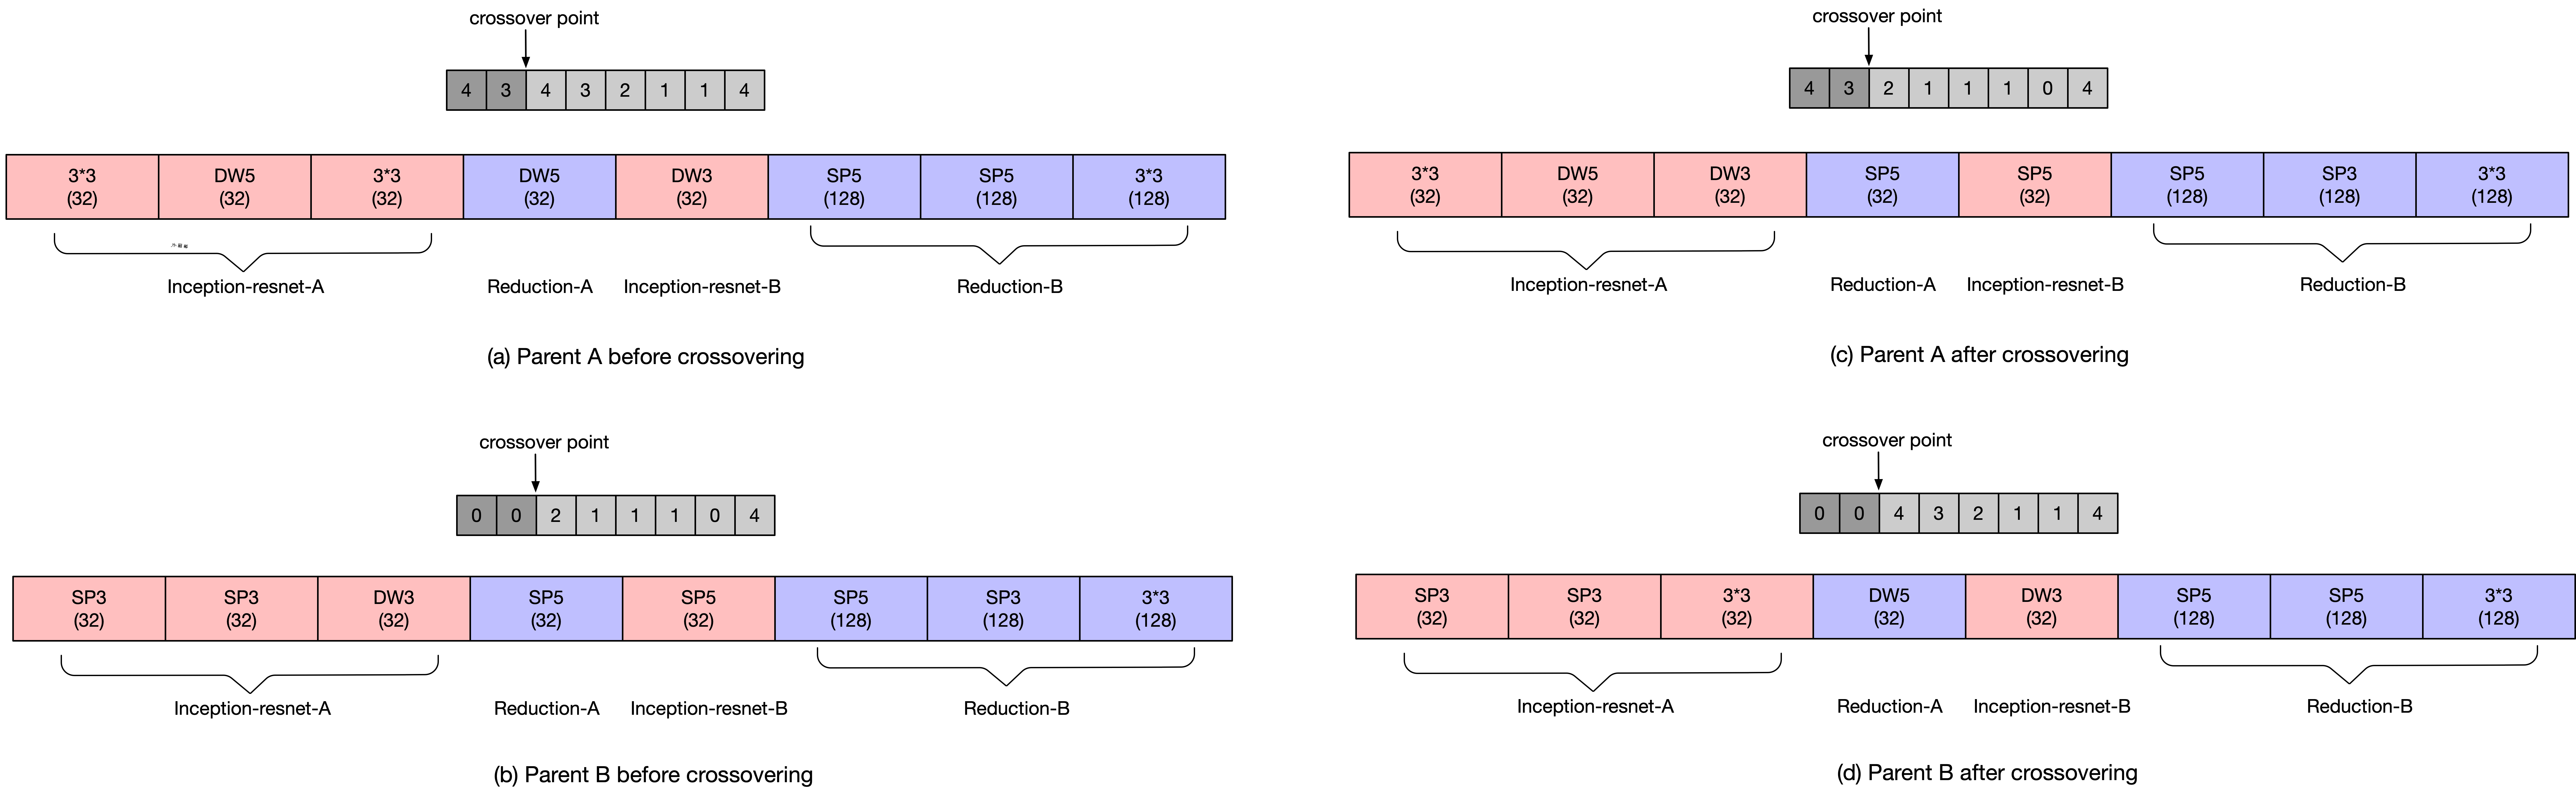
\includegraphics[width=7in]{cnn-cross}
\caption{CNN crossover operation.}
\label{fig_7}
\end{figure*}

\begin{figure*}[!t]
\centering
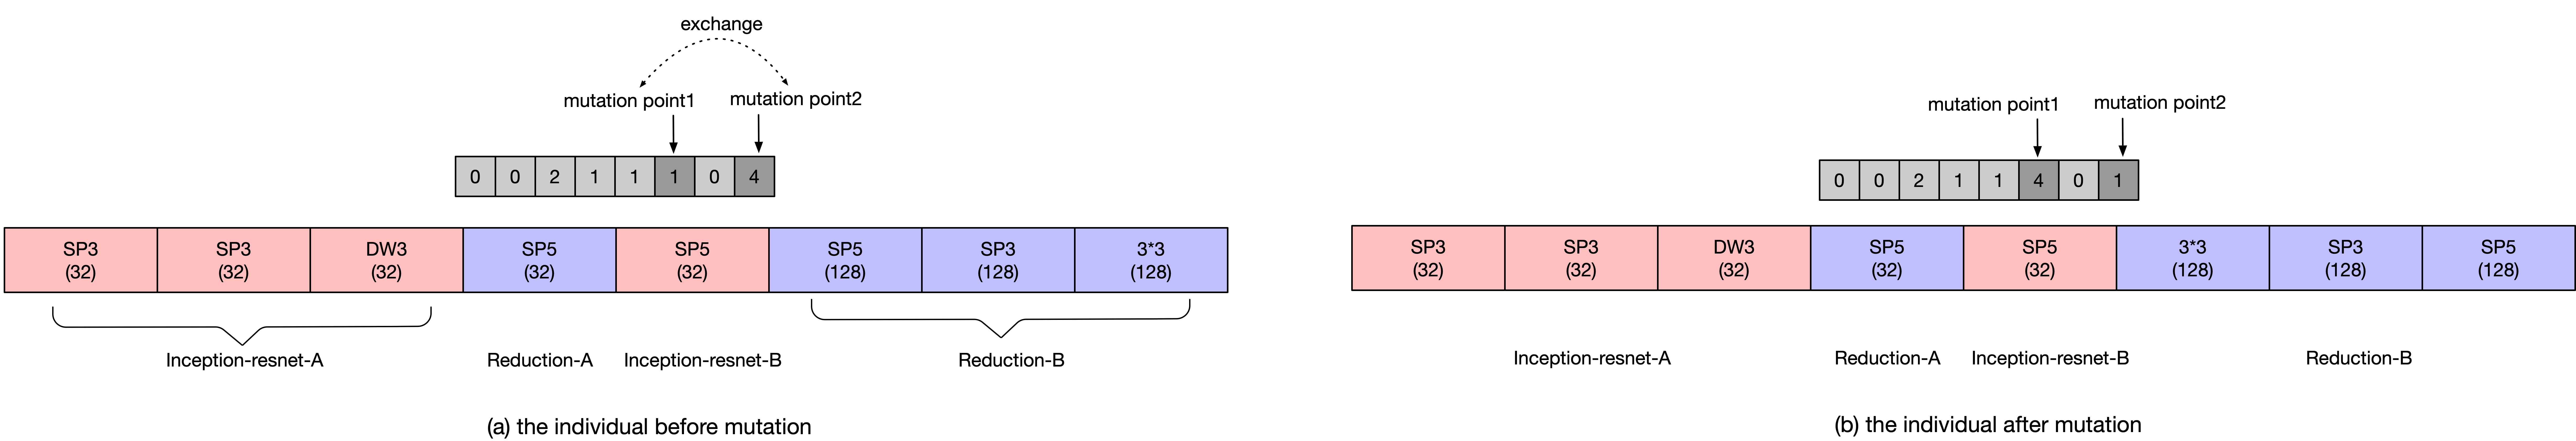
\includegraphics[width=7in]{cnn-mutation}
\caption{CNN mutation operation.}
\label{fig_8}
\end{figure*}

\section{EXPERIMENTAL RESULTS}\label{section_result}
\subsection{Experiment setup and result}
Our network framework consists of GNN block and CNN block, so we need to convert the data into graph data and binary image data according to the above method for adapting to our proposed architecture. Before the two network blocks, there is a reinforcement learning network, which is responsible for dynamically collecting the samples of the input detection model. Our work is based on a publicly available datasets ATTACK \& DEFENSE CHALLENGE 2020 DATASET \cite{74} on IEEE-DATAPORT. The dataset contains two states of vehicle dynamic and stationary, and each part has two types of dataset files: intrusion and normal. In the intrusion file, several intrusion CAN messages are interspersed with normal message. We directly convert these labeled messages into a format that can be the input to the network for training and testing. Our aim is to identify the intrusion CAN messages quickly and accurately from the dataset. Each dataset file has millions of CAN data frames, which can better extract various features in the message. We use the dynamic message part of the vehicle in the dataset, 80\% of the data are used for training and 20\% of the data are used for testing.

The CNN part trains 26 primary generations in advance, each individual trains 200 epochs, and takes the best accuracy as the adaptability index. Then, after 30 generations of crossover and mutation, the best 26 individuals are selected as the parents of the next generation, and so on. Fig. \ref{fig_9} shows the results of 16 generations of precision images. When the evolution process progresses, there are fewer and fewer individuals with low precision, whereas more individuals with better precision have evolved. After evolution the accuracy of every individual reached over 85\%. As shown in Table \ref{table3}. although the accuracy at the end of evolution is almost the same as that of the early generation, in the last generation of evolution, the recognition accuracy of excellent individuals selected after training is 5\% higher than that of the first generation.

\begin{figure}[!t]
\centering
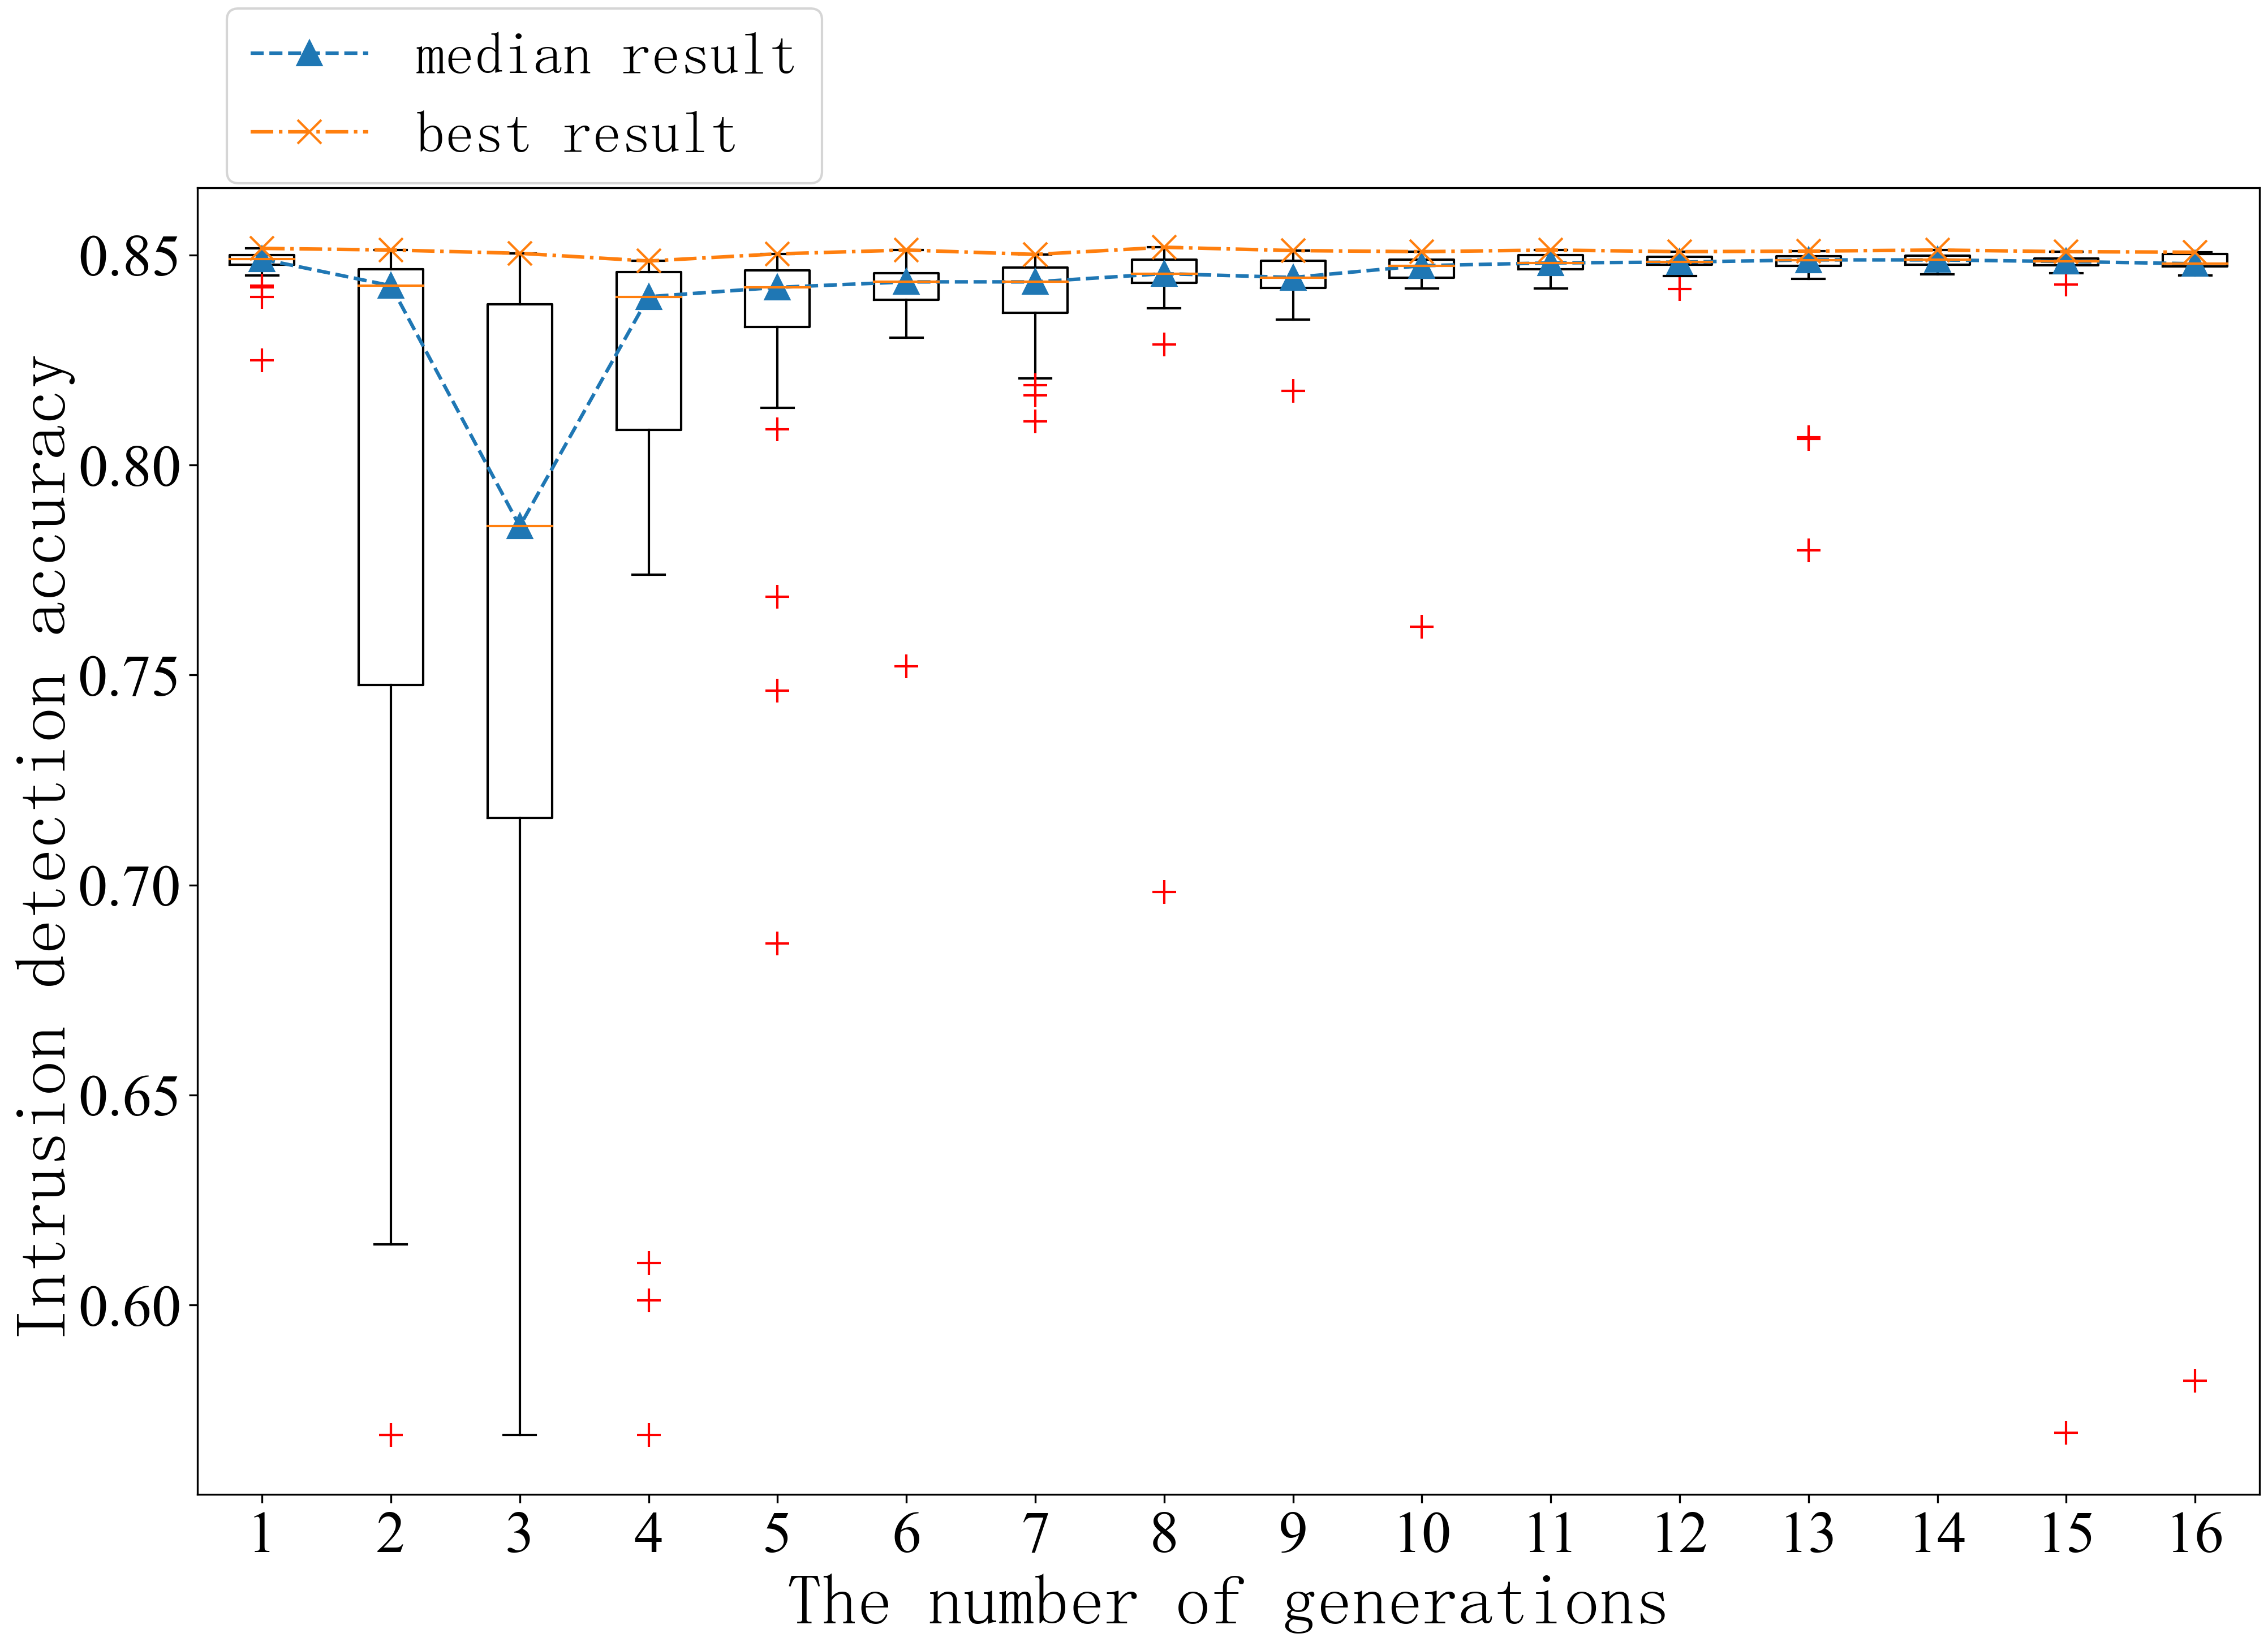
\includegraphics[width=3.5in]{cnn_evo}
\caption{CNN evolution result.}
\label{fig_9}
\end{figure}

\begin{table}[!t]
\caption{Individual comparison between early generation and post evolution\label{table3}}
\centering
\begin{tabular}{cccc}
\hline
stage & gene code & accuracy	 & flops\\
\hline
First Gen &  2,4,2,0,3,4,0,3 &  85.13\% &  2874.5M\\
After evolution without training & 4,4,4,2,3,0,2,3 & 85.15\% & 2628.7M\\
After evolution with training & 4,4,4,2,3,0,2,3 & \textbf{90.20\%} & 2628.7M\\
\hline
\end{tabular}
\end{table}

In the GNN part, first convert the data into graph data, and obtain the prediction results through graph coarsen, GCN, prediction layer, the number of GCN layers and prediction layers of the GNN etc. The neurons of each prediction layer are optimized by EA. At the beginning, 100 primary generations were randomly generated, and 7 individuals at the Pareto front were selected from the primary generation as the parents of the next generation, evolving for 30 generations. The complexity of 30 generations with flops in x-axis, accuracy of error in y-axis is shown in Fig. \ref{fig_10}. Accuracy of error refers to 1 – accuracy (1-acc), so the smaller the accuracy of error, the higher the accuracy.  Flops refers to the number of matrix operations in the process of network recognition. Ther are divided by the number of matrix operations of hypernetwork to convert the flops index into a range of 0 to 1. Red dots are used to identify the last generations of individuals.  The last individuals evolved in the lower left corner of Fig. \ref{fig_10} represent higher accuracy and lower complexity. The Fig. \ref{fig_best_all_gen_gnn} shows the evolution process of GNN and the individuals with the highest accuracy in each generation. It can be seen from the figure that the last generation of individuals have the smallest complexity while ensuring high accuracy.

\begin{figure}[!t]
\centering
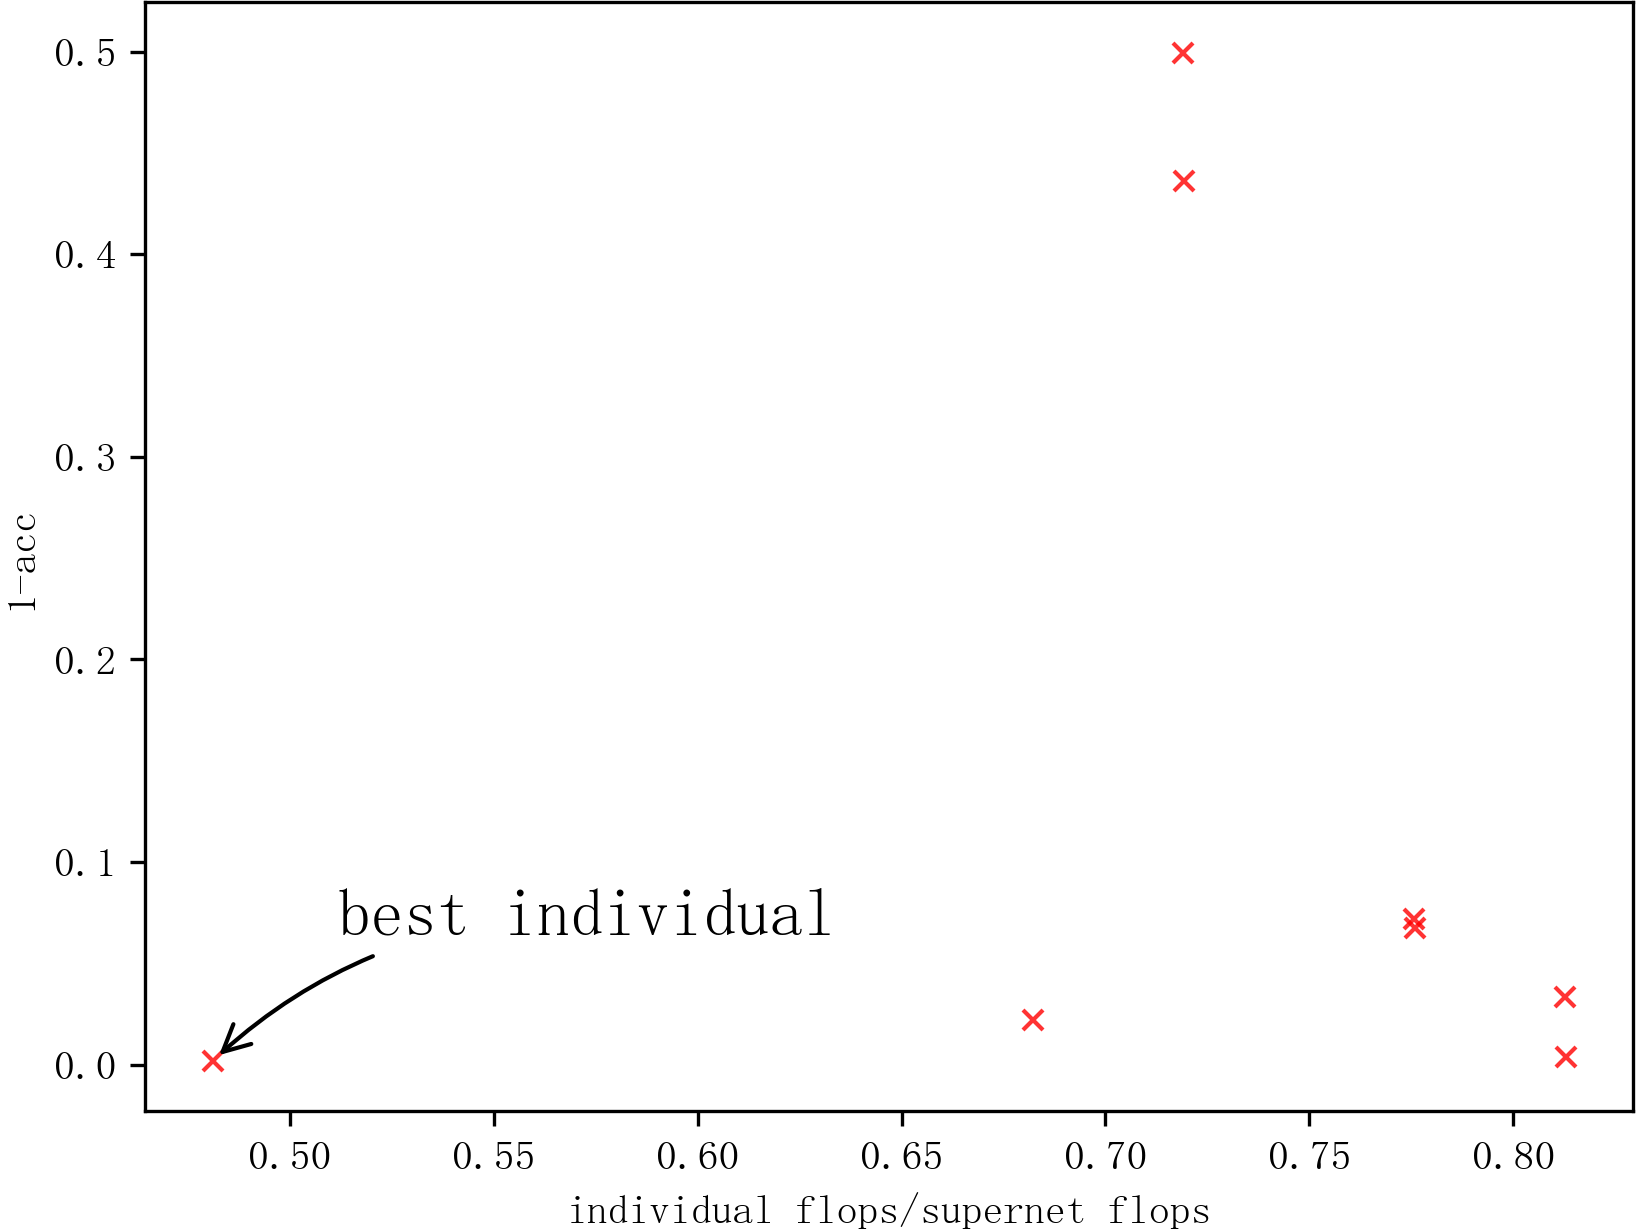
\includegraphics[width=3in]{gnn_evo}
\caption{GNN revolution result.}
\label{fig_10}
\end{figure}

\begin{figure}[!t]
\centering
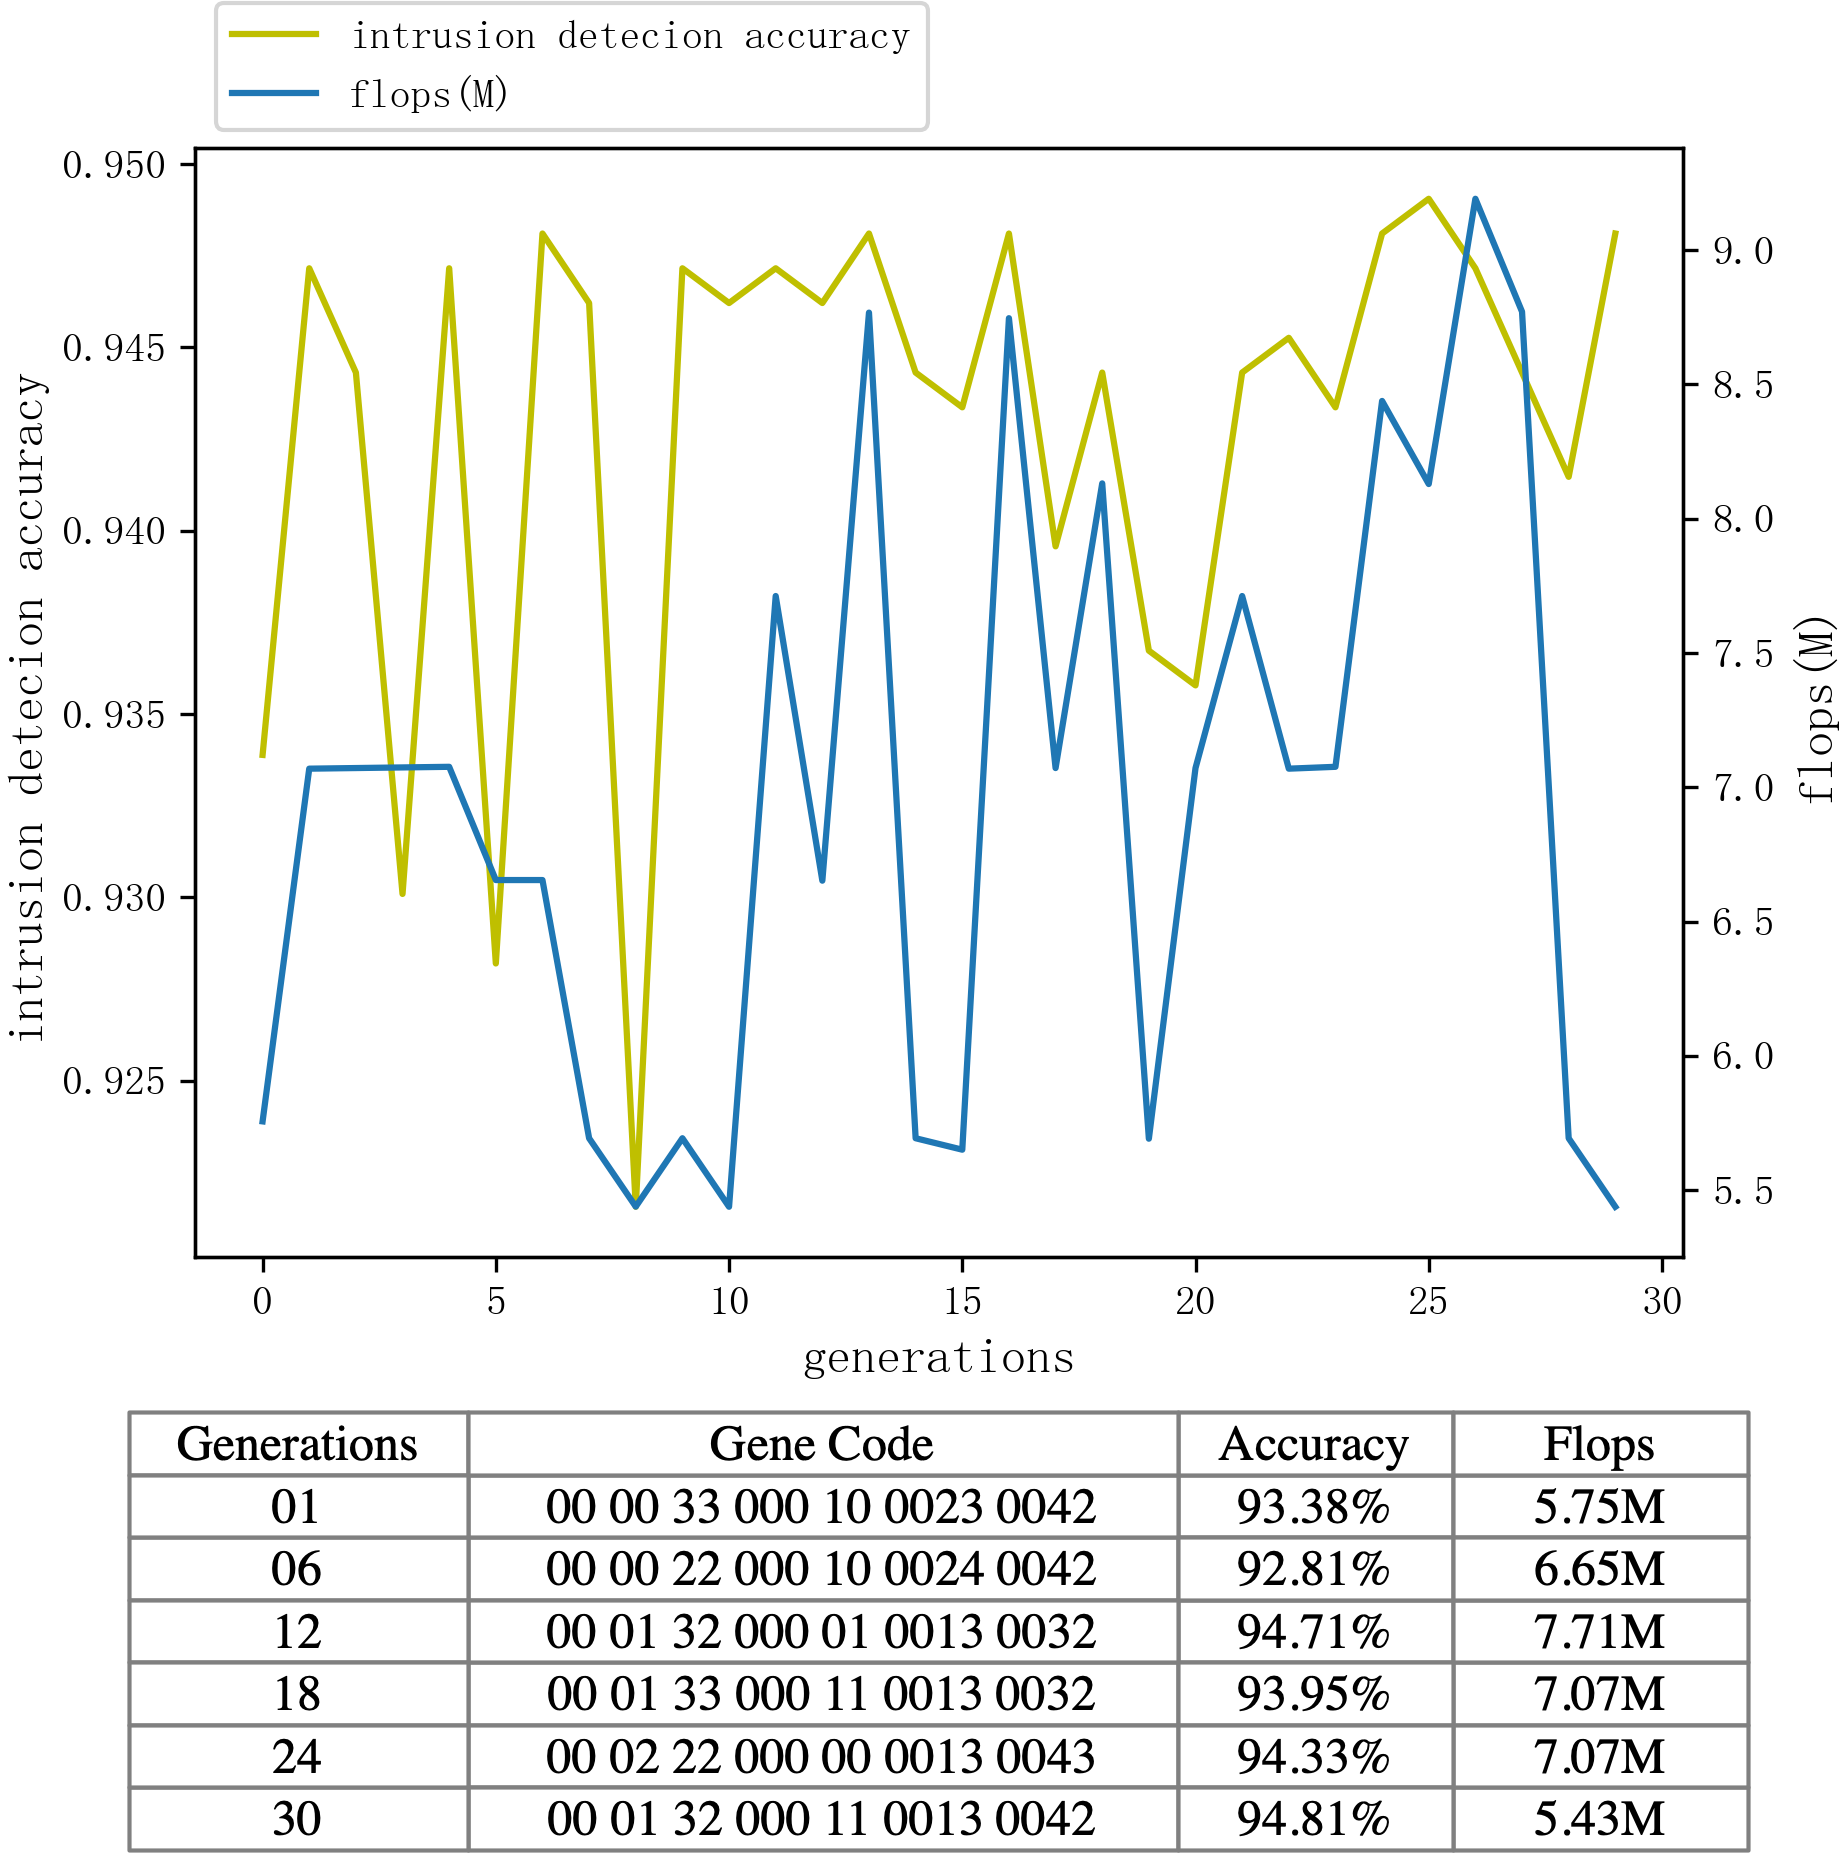
\includegraphics[width=3in]{best_all_gen_gnn}
\caption{In the process of evolution, the individuals with the highest accuracy in each generation and their flops. It can be seen from the figure that the value of flop decreases with the increase of accuracy of intrusion detection.}
\label{fig_best_all_gen_gnn}
\end{figure}

We compared the impact of using the direction information of graph data on Intrusion Detection. The pooling matrix required for graph collapse classification is composed of eigenvectors of the Laplacian matrix of subgraphs. We also compare the impact of Laplacian matrix normalization on intrusion detection. It can be seen from Fig. \ref{fig_11} that the result of using both graph data direction information and Laplace normalization is not the best. Removing the direction information of graph data will make the effect of intrusion detection better, so more use of graph data information will not necessarily improve the results of intrusion detection. Removing the Laplacian matrix normalization will also make the intrusion detection effect better, and reduce the amount of calculations needed for data preprocessing. Therefore, it is reasonable to add the direction information of graph data and the normalization information of Laplace matrix into the search space. The final training results of the three networks can be seen from the Table \ref{table4}.


\begin{figure}[!t]
\centering
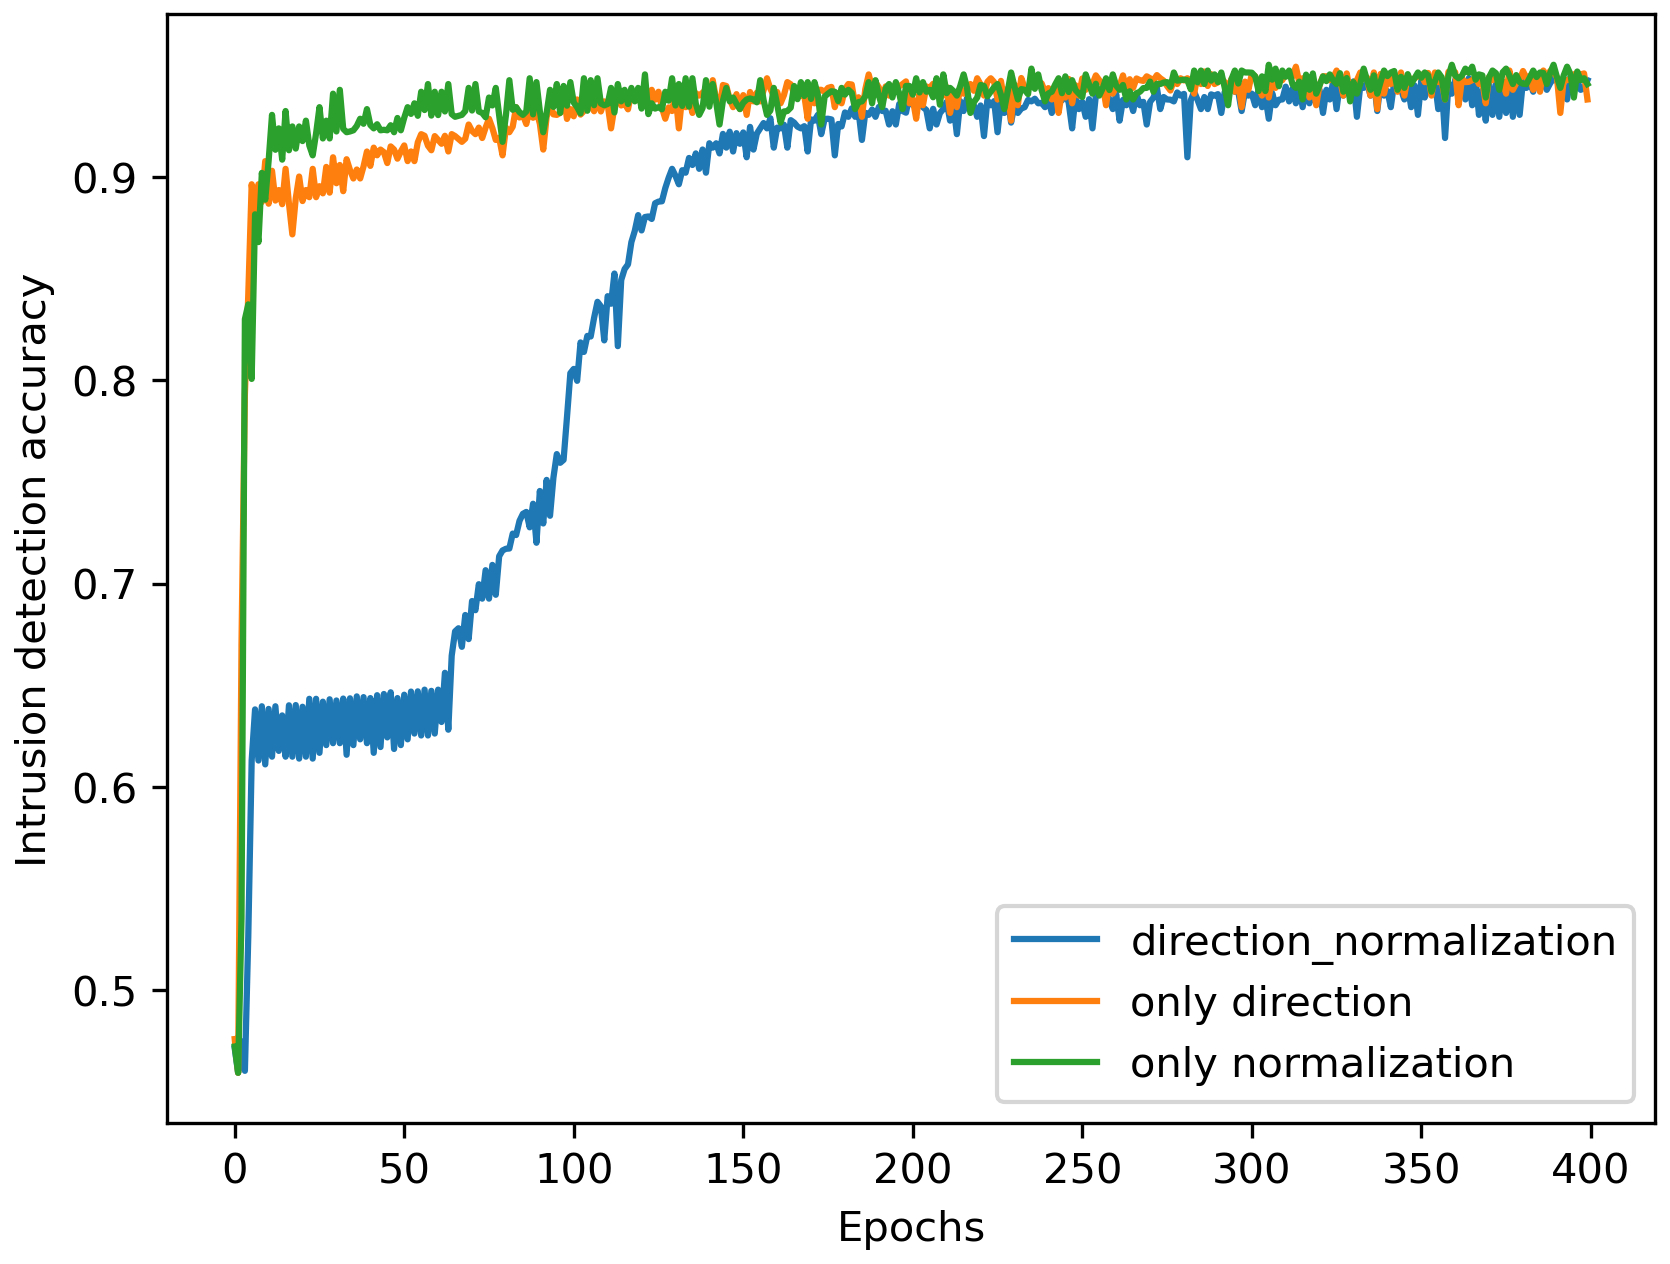
\includegraphics[width=3in]{di_nor_01}
\caption{The impact of graph data processing on Intrusion Detection. the three lines show the impact of directed/undirected graph and processing normalization/no normalization for subgraph’s laplacian matrices to learning logical feature of CAN. The final results of three individuals described on this figure shown in Table \ref{table4}.}
\label{fig_11}
\end{figure}

\begin{table}[!t]
\caption{comparison results of three GNNs\label{table4}}
\centering
\begin{tabular}{ccc}
\hline
contrast factor & gene code & accuracy\\
\hline
direction\_normalization & 1100 0000 000 0021 0124 &  94.86\%\\
only direction & 1000 0000 000 0021 0124 & 95.43\%\\
only normalization & 0100 0000 000 0021 0124 & 95.52\%\\
\hline
\end{tabular}
\end{table}

\subsection{Compare with other deep learning method}
This experiment compares the experimental results of our method with LSTM, DNN, CNN and GNN. Taylor in \cite{49} uses LSTM and Fully Connected Neural Network to extract the timing features of the data part of CAN. However, each CANID needs to train a complete neural network separately, so it is computationally expensive. The loss function of the network is defined as the CrossEntropy loss of each bit corresponding to two adjacent frames of CAN messages. In the network verification stage, the maximum loss value of all bits is used as the basis for whether it is an intrusion message. The publicly available Car Hacking Challenge Dataset rev20Mar2021 \cite{74}, is used for training and verifying the neural network. They use the normal message part to train the LSTM network, and then use the data mixed with the abnormal messages to test the network. We find that good results can be obtained after a small number of epochs. It is mentioned in the paper that some bits with low change frequency can be ignored by analyzing the data segment of CAN ID. Kang et al. \cite{75} additionally employ the 64-bit data segment of CAN messages to feed the bit stream into the DNN network directly. The advantage of this network, not discussed in detail in this paper, is that it is more efficient and can be directly input the network without data processing. We adopt five layers of fully connected layers. The first layer has 64 neurons to receive 64 bits CAN messages bitstream, the second layer has 128 neurons, the third layer has 512 neurons, the fourth layer has 256 neurons, the fifth layer has 32 neurons, and the sixth layer outputs the second classification. Through the verification of public dataset, the accuracy is low, but the neural network is simple and does not need data preprocessing. Song et al. \cite{48} uses a similar convolutional network component to ours. We utilize our network framework directly. The identical design as described in the study may be directly constructed using the gene "44440444". The dataset in \cite{48} was gathered by the author themselves. The classification accuracy of the public dataset does not match that of the author's own experiment, which is lower than that of the MOEA-evolved convolution network. Our algorithm combines the two advantages of the spatial feature extraction of CNN and the logical feature of GNN, compares the difference of two-dimensional variables output by the two networks when outputting the results, and takes the network result with large difference as the final result, which is the result of taking a network that is more confident in the intrusion detection. Using this method, the two forms of networks can complement each other. Table \ref{table5} shows the comparison result of these network architectures. It can be seen that our network can achieve 98.87\% the highest recognition accuracy, which is extremely necessary for cyber security. From the results, it can be seen that the accuracy of a single GNN network is lower than that of the combination of two networks.

\subsection{Limitations of the Proposed Model}
\begin{enumerate}
\item{Although we use MOEA to optimize GNN of our model, the computational complexity of the proposed model combining RL, CNN and GNN, is higher than that of the previous work. The CNN has the highest computational complexity among the three neural networks. However, our model does indeed obtain the best accuracy of intrusion detection of CAN.}
\item{Converting the original CAN message into binary image and graph data is needed for intrusion detection of CNN and GNN. Therefore, compared with the LSTM [75] which directly input the CAN messages, our method needs additional data preprocessing.}
\item{CNN and GNN should detect the same CAN message at the same time. However, their detection system is slightly asynchronous by nature. For example, CNN can only recognize multiple frames of 29 for each packet, whereas the GNN accepts the entire packet as input. This leads to a minor error in CNN intrusion detection.}
\end{enumerate}

\begin{table}[!t]
\caption{CNN search space\label{table5}}
\centering
\begin{tabular}{cc}
\hline
deep learning method & accuracy\\
\hline
LSTM\cite{49} & 97.02\%\\
DNN\cite{75} & 95.36\%\\
GNN & 96.43\%\\
CNN\cite{48} & 85.06\%\\
our method without RL & 95.17\%\\
our method with RL & \textbf{99.87\%}\\
\hline
\end{tabular}
\end{table}

\section{CONCLUSION AND FUTURE WORK}\label{section_conclusion}
We propose an intrusion detection model in the vehicle control area network based on a lower complexity deep neural network and increased accuracy using a multi-objective evolutionary algorithm assisted neural architecture search. As far as we know, GNN is used for CAN intrusion detection for the first time in this work, and detection results of GNN alone can reach more than 95\%. We also combine the dual advantages of GNN and CNN in this work. The detection results of the two networks are complementarily used. In addition, CAN's logical and spatial properties are also employed. Although it can achieve pretty good recognition accuracy, compared with the previously published work, the computational complexity of our network is slightly higher. Evolutionary algorithms (EAs) are critical in the future and exhibit great promise in asynchronous computing systems in terms of cost and reliability. We may expand our proposed EAs to significantly simplify network design by developing a more extensive search space. A combination model of GNN and LSTM (replacing computationally expensive CNN) can be considered to reduce model’s complexity. It can be considered to search the overall architecture of RL, CNN and GNN concurrently, so as to improve the detection accuracy and reduce the complexity. Future research may also attempt to increase the number of MOEA objective functions, e.g., false-positive and true positive rates, to produce a more robust intrusion detection model.

%\section*{Acknowledgments}
%This should be a simple paragraph before the References to thank those individuals and institutions who have supported your work on this article.



%{\appendix[Proof of the Zonklar Equations]
%Use $\backslash${\tt{appendix}} if you have a single appendix:
%Do not use $\backslash${\tt{section}} anymore after $\backslash${\tt{appendix}}, only $\backslash${\tt{section*}}.
%If you have multiple appendixes use $\backslash${\tt{appendices}} then use $\backslash${\tt{section}} to start each appendix.
%You must declare a $\backslash${\tt{section}} before using any $\backslash${\tt{subsection}} or using $\backslash${\tt{label}} ($\backslash${\tt{appendices}} by itself
% starts a section numbered zero.)}



%{\appendices
%\section*{Proof of the First Zonklar Equation}
%Appendix one text goes here.
% You can choose not to have a title for an appendix if you want by leaving the argument blank
%\section*{Proof of the Second Zonklar Equation}
%Appendix two text goes here.}



%\section{References Section}
%You can use a bibliography generated by BibTeX as a .bbl file.
% BibTeX documentation can be easily obtained at:
% http://mirror.ctan.org/biblio/bibtex/contrib/doc/
% The IEEEtran BibTeX style support page is:
% http://www.michaelshell.org/tex/ieeetran/bibtex/
 
 % argument is your BibTeX string definitions and bibliography database(s)
%\bibliography{IEEEabrv,../bib/paper}
%
%\section{Simple References}
%You can manually copy in the resultant .bbl file and set second argument of $\backslash${\tt{begin}} to the number of references
% (used to reserve space for the reference number labels box).

\bibliography{paper}
\bibliographystyle{IEEEtran}


%\newpage
%
%\section{Biography Section}
%If you have an EPS/PDF photo (graphicx package needed), extra braces are
% needed around the contents of the optional argument to biography to prevent
% the LaTeX parser from getting confused when it sees the complicated
% $\backslash${\tt{includegraphics}} command within an optional argument. (You can create
% your own custom macro containing the $\backslash${\tt{includegraphics}} command to make things
% simpler here.)
% 
%\vspace{11pt}
%
%%\bf{If you include a photo:}\vspace{-33pt}
%%\begin{IEEEbiography}[{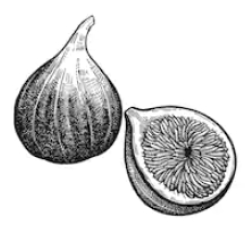
\includegraphics[width=1in,height=1.25in,clip,keepaspectratio]{fig1}}]{Michael Shell}
%%Use $\backslash${\tt{begin\{IEEEbiography\}}} and then for the 1st argument use $\backslash${\tt{includegraphics}} to declare and link the author photo.
%%Use the author name as the 3rd argument followed by the biography text.
%%\end{IEEEbiography}
%
%\vspace{11pt}
%
%\bf{If you will not include a photo:}\vspace{-33pt}
%\begin{IEEEbiographynophoto}{John Doe}
%Use $\backslash${\tt{begin\{IEEEbiographynophoto\}}} and the author name as the argument followed by the biography text.
%\end{IEEEbiographynophoto}
%
%
%
%
%\vfill

\end{document}